\documentclass[usenames,dvipsnames,11pt,pdf,utf8,russian,aspectratio=43]{beamer}
\usepackage{cmap}
\usepackage[T2A]{fontenc}
\usepackage[english,russian]{babel}
\usepackage{subfig}
\usepackage{color}
\usepackage{multicol}
\usepackage{appendixnumberbeamer}
\usepackage{multicol}
\usepackage{tikz}
\usepackage{mathbbol}
\usepackage{amssymb}   
\usepackage{xargs}             % AMS Math
\DeclareUnicodeCharacter{00A0}{ } % При наборе текста с планшета появляются невидимые символы. ЭТо костыль.

\DeclareSymbolFontAlphabet{\mathbb}{AMSb}%
\DeclareSymbolFontAlphabet{\amsmathbb}{bbold}%


\usetikzlibrary{arrows,automata}
\usetikzlibrary{positioning}



\DeclareMathOperator*{\argmin}{arg\,min}

\DeclareMathOperator*{\argmax}{arg\,max}
%
% Choose how your presentation looks.
%
% For more themes, color themes and font themes, see:
% http://deic.uab.es/~iblanes/beamer_gallery/index_by_theme.html
%
\mode<presentation>
{
  \usetheme{Boadilla}      % or try Darmstadt, Madrid, Warsaw, ...
  \usecolortheme{seagull} % or try albatross, beaver, crane, ..

  \usefonttheme{structurebold}  % or try serif, structurebold, ...
  \setbeamertemplate{navigation symbols}{}
  \setbeamertemplate{caption}[numbered]

} 
\setbeamercolor{mygray}{fg=gray,bg=white}


\setbeamertemplate{footline}
{
  \leavevmode%
  \hbox{%
  \begin{beamercolorbox}[wd=.9\paperwidth,ht=2.25ex,dp=1ex,center]{}%
   
  \end{beamercolorbox}%
  \begin{beamercolorbox}[wd=.1\paperwidth,ht=2.25ex,dp=1ex]{mygray}%
   
    \insertframenumber{} / \inserttotalframenumber\hspace*{1ex}
  \end{beamercolorbox}}%
  \vskip0pt%
}



\captionsetup[subfloat]{labelformat=empty}
\title[Model structure selection]{Bayesian selection of \\deep learning model structure}
\author{Oleg Bakhteev}



\institute[]{Supervisor: Prof. Vadim Strijov\\}  
   
%\institute[МФТИ]{Московский Физико-Технический Институт (Государственный Университет)}
\date[2019]{Moscow Institute of Physics and Technology\\November 21, 2019}
\begin{document}
% nb: очень не люблю макросы. Но что поделать 
% https://stackoverflow.com/questions/1509799/how-to-replace-latex-macros-with-their-definitions-using-latex
\newcommand{\D}{\mathfrak{D}}
\newcommand{\x}{\mathbf{x}}
\newcommand{\X}{\mathbf{X}}
\newcommand{\y}{\mathbf{y}}
\newcommand{\Xb}{\mathbb{X}}
\newcommand{\yb}{\mathbb{Y}}
\newcommand{\F}{\mathfrak{F}}



\newcommand{\w}{\mathbf{w}}
\newcommand{\Wb}{\mathbb{W}}
\newcommand{\Uw}{U_\mathbf{w}}

\newcommand{\Gam}{\boldsymbol{\Gamma}}
\newcommand{\Gb}{\amsmathbb{\Gamma}}
\newcommand{\UG}{U_{\boldsymbol{\Gamma}}}

\newcommand{\h}{\mathbf{h}}
\newcommand{\Hb}{\mathbb{H}}
\newcommand{\Uh}{U_{\mathbf{h}}}

\newcommand{\teta}{\boldsymbol{\theta}}
\newcommand{\Tetab}{\amsmathbb{\Theta}}
\newcommand{\Uteta}{U_{\boldsymbol{\theta}}}

\newcommand{\tetaw}{\boldsymbol{\theta}_\mathbf{w}}
\newcommand{\Tetawb}{\amsmathbb{\Theta}_\mathbf{w}}
\newcommand{\Utetaw}{U_{\boldsymbol{\theta}_\mathbf{w}}}
\newcommand{\tetaG}{\boldsymbol{\theta}_{\boldsymbol{\Gamma}}}
\newcommand{\TetaGb}{\amsmathbb{\Theta}_{\boldsymbol{\Gamma}}}
\newcommand{\UtetaG}{U_{\boldsymbol{\theta}_{\boldsymbol{\Gamma}}}}

\newcommand{\lam}{\boldsymbol{\lambda}}
\newcommand{\Lamb}{\amsmathbb{\Lambda}}
\newcommand{\Ulam}{U_{\boldsymbol{\lambda}}}

%\newcommand{\prior}{p(\mathbf{w}, \boldsymbol{\Gamma}|\mathbf{h},\boldsymbol{\lambda})}
\newcommandx{\prior}[4][1=\mathbf{w},2=\boldsymbol{\Gamma},3=\mathbf{h},4=\boldsymbol{\lambda},usedefault]{p(#1,#2|#3,#4)}
\newcommandx{\priorh}[2][1=\mathbf{h}, 2=\boldsymbol{\lambda},usedefault]{p(#1|#2)}
\newcommandx{\priorG}[3][1=\boldsymbol{\Gamma}, 2= \mathbf{h}, 3=\boldsymbol{\lambda},usedefault]{p(#1|#2,#3)}
\newcommandx{\priorw}[4][1=\mathbf{w},2=\boldsymbol{\Gamma},3=\mathbf{h},4=\boldsymbol{\lambda},usedefault]{p(#1|#2,#3,#4)}


\newcommand{\post}{p(\mathbf{w}, \boldsymbol{\Gamma}|\mathbf{y}, \mathbf{X}, \mathbf{h},\boldsymbol{\lambda})}
\newcommand{\posth}{p(\mathbf{h}|\mathbf{y}, \mathbf{X},\boldsymbol{\lambda})}
\newcommand{\postG}{p(\boldsymbol{\Gamma}|\mathbf{y}, \mathbf{X}, \mathbf{h},\boldsymbol{\lambda})}
\newcommand{\postw}{p(\mathbf{w}|\mathbf{y}, \mathbf{X}, \boldsymbol{\Gamma}, \mathbf{h},\boldsymbol{\lambda})}


\newcommandx{\q}[1][1=\boldsymbol{\theta}, usedefault]{q(\mathbf{w}, \boldsymbol{\Gamma}|#1)}
\newcommandx{\qG}[2][1=\boldsymbol{\Gamma},2=\boldsymbol{\theta}_{\boldsymbol{\Gamma}},usedefault]{q_{\boldsymbol{\Gamma}}(#1|#2)}
\newcommandx{\qw}[3][1=\mathbf{w}, 2=\boldsymbol{\Gamma},3=\boldsymbol{\theta}_\mathbf{w},usedefault]{q_\mathbf{w}(#1|#2,#3)}


\newcommandx{\LL}[4][1=\mathbf{y},2=\mathbf{X},3=\mathbf{w},4=\boldsymbol{\Gamma},usedefault]{p(#1|#2,#3,#4)}

\newcommand{\EV}{p(\mathbf{y}|\mathbf{X}, \mathbf{h},\boldsymbol{\lambda})}

\newcommandx{\Loss}[5][1=\boldsymbol{\theta},2=\mathbf{y},3=\mathbf{X},4=\mathbf{h},5=\boldsymbol{\lambda},usedefault]{L(#1 |#2,#3,#4,#5)}
\newcommandx{\Val}[5][1=\mathbf{h},2=\mathbf{y},3=\mathbf{X},4=\boldsymbol{\theta},5=\boldsymbol{\lambda},usedefault]{Q(#1|#2,#3,#4,#5)}

% прочее
\newcommand{\model}{\mathbf{f}}
\newcommand{\A}{\mathbf{A}}
\newcommand{\s}{\mathbf{s}}
\newcommand{\g}{\boldsymbol{\gamma}}
\newcommand{\E}{\mathsf{E}}
\newcommand{\KL}[2]{D_\text{KL}\bigl(#1 || #2\bigr)}

\newcommand{\lamT}{\lambda_{\text{temp}}}
\newcommand{\lamLL}{\lambda_\text{likelihood}^\text{Q}}
\newcommand{\lamCL}{\lambda_\text{prior}^\text{L}}
\newcommand{\lamCQ}{\lambda_\text{prior}^\text{Q}}
\newcommand{\lamS}{\boldsymbol{\lambda}_\text{struct}^\text{Q}}
\newcommandx{\TLoss}[6][1=\boldsymbol{\theta},2=L,3=\mathbf{y}, 4=\mathbf{X}, 5=\mathbf{h},6=\boldsymbol{\lambda},usedefault]{T(#1|#2,#3,#4,#5,#6)}
\newcommandx{\TVal}[6][1=\mathbf{h},2=Q,3=\mathbf{y}, 4=\mathbf{X}, 5=\boldsymbol{\teta},6=\boldsymbol{\lambda},usedefault]{T(#1|#2,#3,#4,#5,#6)}
%\newcommand{\log}{\text{log}~}




\begin{frame}
  \titlepage
\end{frame}



\begin{frame}{Selection of deep learning model structure}
\small
\textbf{Goal :} to propose a method of selection of deep learning model structure.\\
\textbf{Objectives:}
\begin{enumerate}
\item Proposal of suboptimal and optimal complexity criteria for deep learning models.
\item Proposal of an algorithm suboptimal deep learning model selection and optimization of model parameters.
\end{enumerate}
\textbf{Investigated problems}
\begin{enumerate}
\item Large number of parameters and hyperparameters, high computational complexity.
\item Multiextremality and non-convexity of optimization.
\end{enumerate}
\textbf{Methods}\\
A deep learning model is considered as a multigraph. For the suboptimal model selection we use a composition of methods of automatic relevance determination and hyperparameter gradient optimization methods.
\end{frame}



\begin{frame}    
                                                                                                                        
\frametitle{Model structure selection challenge}     
Data likelihood does not change with removing redundant parameters.
\begin{figure}[h]                                                                                                                               
\centering                                                                                                                                      
\subfloat[Redundancy of model parameters]{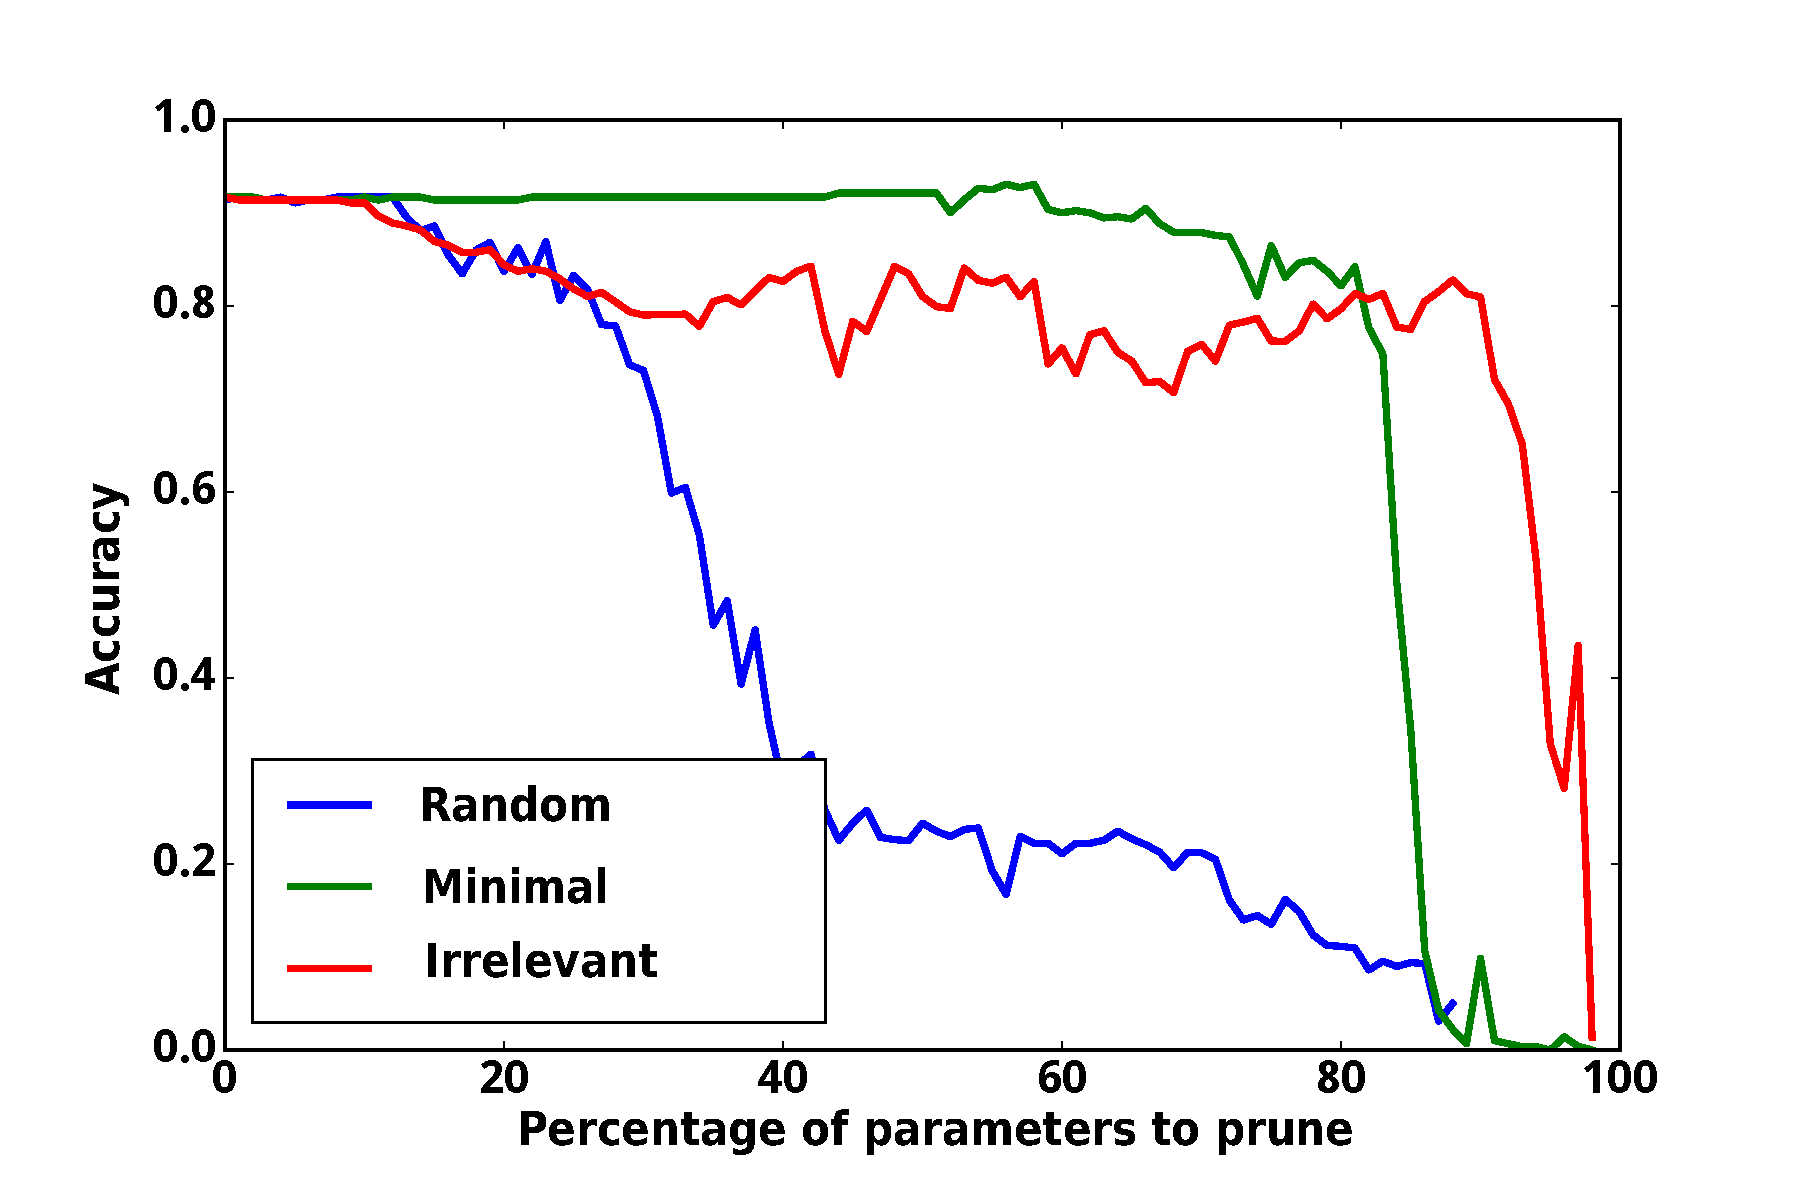
\includegraphics[width=0.55\textwidth]{./slide_plots/pruning_eng.pdf}}   
\hspace*{-1cm}                                       
\subfloat[Model robustness]{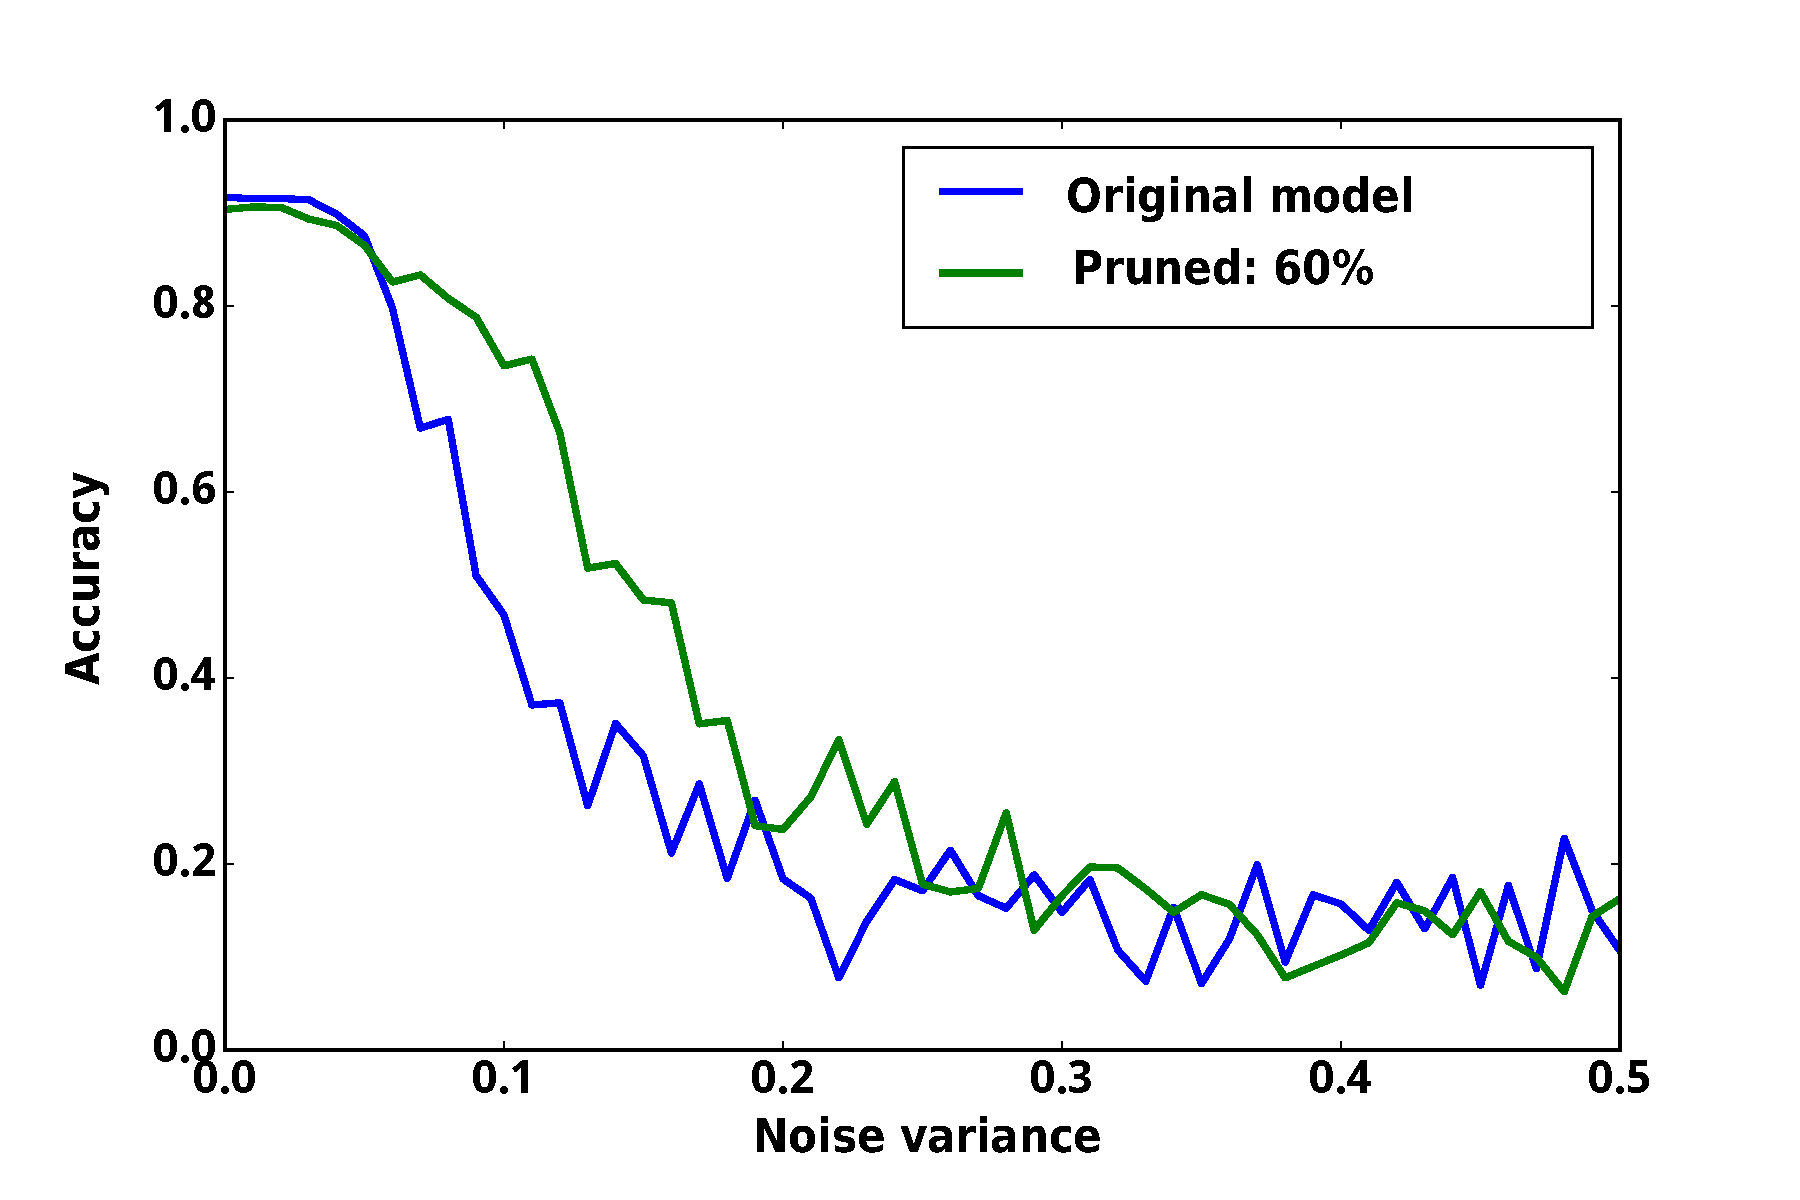
\includegraphics[width=0.55\textwidth]{./slide_plots/noise_en.pdf}}                                                     
\end{figure}                                                                                                   
\textcolor{gray}{Deep learning models have implicitly redundant complexity.}  

                                                                                                                                             
\end{frame}    

\begin{frame}{Deep learning model}
\small
\begin{block}{Definition}
\textit{Model} $\mathbf{f}(\mathbf{w}, \mathbf{x})$ is a differentiable function with respect to parameters $\mathbf{w}$  from the set of object descriptions into the set of labels:
\[
    \mathbf{f}: \mathbb{X} \times \mathbb{W} \to \mathbb{Y},
\] 
where $\mathbb{W}$ is a space of parameters of model $\mathbf{f}$.
\end{block}
~\\
\textbf{Main challenge} of deep learning model selection is in large number of parameters of models. This disallows to use many classical approached for the model and structure selection (AIC, BIC, cross-validation). \\~\\
A model is defined by its parameters $\mathbf{W}$ and structure $\boldsymbol{\Gamma}$.\\
A \textbf{structure} defines a set of functional superpositions in the model. It is selected using statistical complexity criteria.\\

\textbf{Empirical model complexity estimations:}
\begin{enumerate}
\item number of parameters;
\item number of superpositions in the model.
\end{enumerate}
\end{frame}


\begin{frame}{Structure selection: one-layer network}
\small
The model $\mathbf{f}$ is defined by the \textbf{structure}  $\boldsymbol{\Gamma} = [\boldsymbol{\gamma}^{0,1}, {\boldsymbol{\gamma}^{1,2}}].$

\[
    \text{Model: }\mathbf{f}(\mathbf{x}) = \textbf{softmax}\left((\mathbf{w}^{1,2}_0)^\mathsf{T}{\mathbf{f}_1}(\mathbf{x})\right), \quad \mathbf{f}(\mathbf{x}): \mathbb{R}^n \to [0,1]^{|\mathbb{Y}|}, \quad \mathbf{x} \in \mathbb{R}^n.
\]
\[
\mathbf{f}_1(\mathbf{x}) = {\gamma}^{0,1}_{0}\mathbf{g}^{0,1}_{0}(\mathbf{x}) + {\gamma}^{0,1}_{1}\mathbf{g}^{0,1}_{1}(\mathbf{x}),
\]
where $\mathbf{w} = [\mathbf{w}^{0,1}_0, \mathbf{w}^{0,1}_1, \mathbf{w}^{1,2}_0]^{\text{T}}$ --- parameter matrices, $\{\mathbf{g}^{0}_{0,1},\mathbf{g}^{1}_{0,1},{\mathbf{g}^{0}_{1,2}\}}$ --- generalized-linear functions, alternatives of layers of the network.

\begin{tikzpicture}[node distance=0.5cm, auto]
  %\tikzstyle{every state}=[fill=red,draw=none,text=white]

  \node (f0)  at (1,6)                  {$\mathbf{f}_0(\mathbf{x}) = \mathbf{x}$};
  %\node (g11) at (6,3)                    {$\mathbf{g}^{1,1}(\mathbf{x})$};% = \text{Conv}(\mathbf{x}, 3, 32, 1)$};
  %\node (g12)  at (6,9)                   {$\mathbf{g}^{1,2}(\mathbf{x})$};% = \text{Conv}(\mathbf{x}, 4, 32, 1)$};
  \node (f1)  at (7,6)                 {$\mathbf{f}_1(\mathbf{x})$};% = \gamma^{1,1}\mathbf{g}^{1,1}(\mathbf{x}) +  \gamma^{1,2}\mathbf{g}^{1,2}(\mathbf{x})$};
  %\node (g21) at (12,6)                   {$\mathbf{g}^{2,1}(\mathbf{x})$};% = \boldsymbol{\sigma}(\mathbf{w}^{2,1}\mathbf{x})$};
  \node (f2)  at (12,6)                   {$\mathbf{f}_2(\mathbf{x})$};% = \gamma^{2,1}\mathbf{g}^{2,1}(\mathbf{x})$};
  \path[->]  (f0) edge [bend left=50] node {$\gamma^{0,1}_0\mathbf{g}^{0,1}_0(\mathbf{x}) = \gamma^{0,1}_0\boldsymbol{\sigma}\left((\mathbf{w}^{0,1}_0)^{\mathsf{T}}\mathbf{x}\right)$}(f1);
  \path[->] (f0)  edge[bend right=50] node[below] {$\gamma^{0,1}_1\mathbf{g}^{0,1}_1(\mathbf{x}) = \gamma^{0,1}_1\boldsymbol{\sigma}\left((\mathbf{w}^{0,1}_1)^{\mathsf{T}}\mathbf{x}\right)$}(f1);
  \path[->] (f1)  edge node {$\gamma^{1,2}_0\mathbf{g}^{1,2}_0(\mathbf{x}) = \gamma^{1,2}_0\textbf{softmax}\left((\mathbf{w}^{1,2}_0)^{\mathsf{T}}\mathbf{x}\right)$}(f2);       
  \draw[->] (f1) to (f2);
 
\end{tikzpicture}

\end{frame}


\begin{frame}{Deep learning model structure as a graph}
\footnotesize
Define:
\begin{enumerate}
 \item acyclic graph $(V,E)$;
\item for each edge $(j,k) \in E$: a vector primitive differentiable functions $\mathbf{g}^{j,k} = [\mathbf{g}^{j,k}_0, \dots, \mathbf{g}^{j,k}_{K^{j,k}}]$  with length of $K^{j,k}$;
\item for each vertex $v \in V$: a differentiable aggregation function  $\textbf{agg}_v$.
\item a function $\mathbf{f} = \mathbf{f}_{|V|-1}:$
\begin{equation}
\label{eq:modelfam}
    \mathbf{f}_{v}(\mathbf{w}, \mathbf{x}) = \textbf{agg}_{v}\left(\{ \langle \boldsymbol{\gamma}^{j,k}, \mathbf{g}^{j,k} \rangle \circ  \mathbf{f}_j(\mathbf{x})| j \in \text{Adj}(v_k)\}\right), v \in \{1,\dots,|V|-1\}, \quad \mathbf{f}_0(\mathbf{x}) = \mathbf{x}
\end{equation}
that is a function from  $\mathbb{X}$ into a set of labels $\mathbb{Y}$ for any value of  $\boldsymbol{\gamma}^{j,k} \in [0,1]^{K^{j,k}}$.
\end{enumerate}

\begin{block}{Definition}
A \textit{parametric set of models} $\mathfrak{F}$ is a graph $(V, E)$  with a set of primitive functions $\{\mathbf{g}^{j,k}, (j,k) \in E\}$ and aggregation functions  $\{ \textbf{agg}_v, {v \in V}\}$.
\end{block}
\begin{block}{Statement}
A function $\mathbf{f} \in \mathfrak{F}$ is a model for each  $\boldsymbol{\gamma}^{j,k} \in [0,1]^{K^{j,k}}$.
\end{block}
\end{frame}

      

\begin{frame}{Structure restrictions}
An example of restrictions for structure parameter $\boldsymbol{\gamma}$, $|\boldsymbol{\gamma}| = 3$.
\begin{figure}
 \begin{minipage}[t]{.45\textwidth}
        \centering
%1 limit
\begin{tikzpicture}[%
x={(1.5cm,0cm)},
y={(0cm,1.5cm)},
z={({0.5*cos(45)},{0.5*sin(45)})},
]

\coordinate (A) at (0,0,0); 
\coordinate (B) at (1,0,0) ;
\coordinate (C) at (1,1,0); 
\coordinate (D) at (0,1,0); 
\coordinate (E) at (0,0,1); 
\coordinate (F) at (1,0,1); 
\coordinate (G) at (1,1,1); 
\coordinate (H) at (0,1,1   );

%Ecken
\node[circle,scale=0.5,fill=black,draw=black](Ap) at (0,0,0){};
\node[circle,scale=0.5,fill=black,draw=black](Bp) at (1,0,0){};
\node[circle,scale=0.5,fill=black,draw=black](Cp) at (1,1,0){};
\node[circle,scale=0.5,fill=black,draw=black](Dp) at (0,1,0){};
\node[circle,scale=0.5,fill=black,draw=black](Ep) at (0,0,1){};
\node[circle,scale=0.5,fill=black,draw=black](Fp) at (1,0,1){};
\node[circle,scale=0.5,fill=black,draw=black](Gp) at (1,1,1){};
\node[circle,scale=0.5,fill=black,draw=black](Hp) at (0,1,1){};
\node[left= 1pt of A]{[0,0,0]};
\node[right= 1pt of B]{[1,0,0]};
\node[right= 1pt of C]{[1,1,0]};
\node[left= 1pt of D]{[0,1,0]};
\node[left= 1pt of E]{[0,0,1]};
\node[right= 1pt of F]{[1,0,1]};
\node[right= 1pt of G]{[1,1,1]};
\node[left= 1pt of H]{[0,1,1]};

%Kanten
\draw[] (A)
-- (B)  node[midway, below]{}
-- (C)      node[midway, right]{}
-- (D)  node[midway, above]{}
-- (A)  node[midway, left]{};
\draw[] (B) -- (F) -- (G) -- (C);
\draw[] (G) -- (H) -- (D);
\draw[densely dashed] (A) -- (E) -- (F);
\draw[densely dashed] (E) -- (H);

\end{tikzpicture}
\caption*{Cube vertices}
\end{minipage}
\hfill
 \begin{minipage}[t]{.45\textwidth}
        \centering

%2 limit
\begin{tikzpicture}[%
x={(1.5cm,0cm)},
y={(0cm,1.5cm)},
z={({0.5*cos(45)},{0.5*sin(45)})},
]

\coordinate (A) at (0,0,0); 
\coordinate (B) at (1,0,0) ;
\coordinate (C) at (1,1,0); 
\coordinate (D) at (0,1,0); 
\coordinate (E) at (0,0,1); 
\coordinate (F) at (1,0,1); 
\coordinate (G) at (1,1,1); 
\coordinate (H) at (0,1,1   );

%Ecken
\node[left= 1pt of A]{[0,0,0]};
\node[right= 1pt of B]{[1,0,0]};
\node[right= 1pt of C]{};
\node[left= 1pt of D]{[0,1,0]};
\node[left= 1pt of E]{};
\node[right= 1pt of F]{[1,0,1]};
\node[right= 1pt of G]{[1,1,1]};
\node[left= 1pt of H]{[0,1,1]};

%Kanten
\draw[fill=gray] (A)
-- (B)  node[midway, below]{}
-- (C)      node[midway, right]{}
-- (D)  node[midway, above]{}
-- (A)  node[midway, left]{};
\draw[fill=gray] (B) -- (F) -- (G) -- (C);
\draw[fill=gray] (G) -- (H) -- (D);
\draw[fill=gray] (A) -- (E) -- (F);
\draw[fill=gray] (E) -- (H);
\draw[fill=gray] (D) -- (H) -- (G) -- (C);
\end{tikzpicture}
\caption*{Cube interior}
\end{minipage}
\hfill
 \begin{minipage}[t]{.45\textwidth}
        \centering
%3 limit
\begin{tikzpicture}[%
x={(1.5cm,0cm)},
y={(0cm,1.5cm)},
z={({0.5*cos(45)},{0.5*sin(45)})},
]

\coordinate (A) at (0,0,0); 
\coordinate (B) at (1,0,0) ;
\coordinate (C) at (1,1,0); 
\coordinate (D) at (0,1,0); 
\coordinate (E) at (0,0,1); 
\coordinate (F) at (1,0,1); 
\coordinate (G) at (1,1,1); 
\coordinate (H) at (0,1,1   );

%Ecken
\node[circle,scale=0.5,fill=black,draw=black](Bp) at (1,0,0){};
\node[circle,scale=0.5,fill=black,draw=black](Dp) at (0,1,0){};
\node[circle,scale=0.5,fill=black,draw=black](Ep) at (0,0,1){};
\node[left= 1pt of A]{};
\node[right= 1pt of B]{[1,0,0]};
\node[right= 1pt of C]{};
\node[left= 1pt of D]{[0,1,0]};
\node[left= 1pt of E]{[0,0,1]};
\node[right= 1pt of F]{};
\node[right= 1pt of G]{};
\node[left= 1pt of H]{};

%Kanten
\draw[] (A)
-- (B)  node[midway, below]{}
-- (C)      node[midway, right]{}
-- (D)  node[midway, above]{}
-- (A)  node[midway, left]{};
\draw[] (B) -- (F) -- (G) -- (C);
\draw[] (G) -- (H) -- (D);
\draw[densely dashed] (A) -- (E) -- (F);
\draw[densely dashed] (E) -- (H);

\end{tikzpicture}
\caption*{Simplex vertices}
\end{minipage}
\hfill
 \begin{minipage}[t]{.45\textwidth}
        \centering
%4 limit
\begin{tikzpicture}[%
x={(1.5cm,0cm)},
y={(0cm,1.5cm)},
z={({0.5*cos(45)},{0.5*sin(45)})},
]

\coordinate (A) at (0,0,0); 
\coordinate (B) at (1,0,0) ;
\coordinate (C) at (1,1,0); 
\coordinate (D) at (0,1,0); 
\coordinate (E) at (0,0,1); 
\coordinate (F) at (1,0,1); 
\coordinate (G) at (1,1,1); 
\coordinate (H) at (0,1,1   );

%Ecken
\node[left= 1pt of A]{};
\node[right= 1pt of B]{[1,0,0]};
\node[right= 1pt of C]{};
\node[left= 1pt of D]{[0,1,0]};
\node[left= 1pt of E]{[0,0,1]};
\node[right= 1pt of F]{};
\node[right= 1pt of G]{};
\node[left= 1pt of H]{};

%Kanten
\draw[] (A)
-- (B)  node[midway, below]{}
-- (C)      node[midway, right]{}
-- (D)  node[midway, above]{}
-- (A)  node[midway, left]{};
\draw[] (B) -- (F) -- (G) -- (C);
\draw[] (G) -- (H) -- (D);
\draw[densely dashed] (A) -- (E) -- (F);
\draw[densely dashed] (E) -- (H);
\draw[fill=gray] (B) -- (D) -- (E);


\end{tikzpicture}
\caption*{Simplex interior}
\end{minipage}

\end{figure}

\end{frame}






\begin{frame}{Prior distribution}
\footnotesize   
\begin{columns}
\begin{column}{0.6\textwidth}
   \begin{block}{Definition}
\textit{Prior distribution} for parameters $\mathbf{w}$ and structure $\boldsymbol{\Gamma}$ of model $\mathbf{f}$ is a distribution
$
    \textcolor{red}{p(\mathbf{W}, \boldsymbol{\Gamma}|\mathbf{h},\lam)}: \mathbb{W} \times \amsmathbb{\Gamma} \times \mathbb{H} \to \mathbb{R}^{+}, 
$
where $\mathbb{W}$ is a parameter space, $\amsmathbb{\Gamma}$ is a structure space, $\lam$ is a vector of metaparameters.
\end{block}

\end{column}
\begin{column}{0.4\textwidth}  %%<--- here
    \begin{center}
     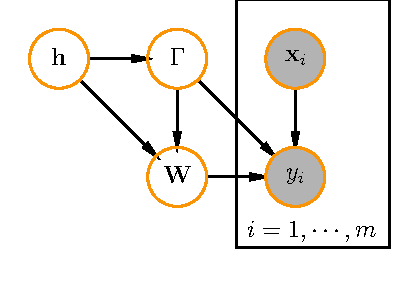
\includegraphics[width=\textwidth]{simple_plate.pdf}
     \end{center}
\end{column}
\end{columns}
\vspace*{-0.5cm}
\begin{block}{Definition}
\textit{Hyperparameters} $\mathbf{h}\in \mathbb{H}$ are the parameters of prior distribution $p(\mathbf{w}, \boldsymbol{\Gamma}|\mathbf{h},\mathbf{f})$ (parameters of the distribution of the parameters and structure  of model $\mathbf{f}$).
 
\end{block}
A model $\mathbf{f}$ is defined by:
\begin{itemize}
\item \textbf{Parameters} $\mathbf{w} \in \mathbb{W}$ that define superpositions  $\mathbf{f}_v$ in the model $\mathbf{f}$.
\item \textbf{Structure} $\boldsymbol{\Gamma}=\{\gamma^{j,k}\}_{(j,k)\in E} \in \amsmathbb{\Gamma}$ that define the contribution of all the superpositions  $\mathbf{f}_v$ into $\mathbf{f}$.
\item \textbf{Hyperparameters} $\mathbf{h} \in \mathbb{H}$ that define the prior distribution.
\item \textbf{Metaparameters} $\boldsymbol{\lambda} \in \amsmathbb{\Lambda}$ that define the optimization function.
\end{itemize}

\end{frame}






\begin{frame}{Prior distribution for the model structure}
Every point in a simplex defines a model.

\textbf{Gumbel-Softmax distribution: }$\textcolor{red}{\boldsymbol{\Gamma}\sim \text{GS}(\mathbf{s}, \lambda_\text{temp})}$\\
\begin{figure}
 \begin{minipage}[t]{.3\textwidth}
        \centering
\begin{tikzpicture}[%
x={(1.7cm,0cm)},
y={(0cm,1.7cm)},
]

\coordinate (A) at (0,0); 
\coordinate (B) at (1,0) ;
\coordinate (C) at (0.5,0.86); 

%Ecken
\node[circle,scale=0.5,fill=black,draw=black](Ap) at (0,0){};
\node[circle,scale=0.5,fill=black,draw=black](Bp) at (1,0){};
\node[circle,scale=0.5,fill=black,draw=black](Cp) at (0.5,0.86){};

%Kanten
\draw[] (A)
-- (B)  node[midway, below]{}
-- (C)      node[midway, right]{}
-- (A)  node[midway, left]{};

\end{tikzpicture}
\caption*{$\lambda_\text{temp}\to0$}
\end{minipage}
\hfill
 \begin{minipage}[t]{.3\textwidth}
   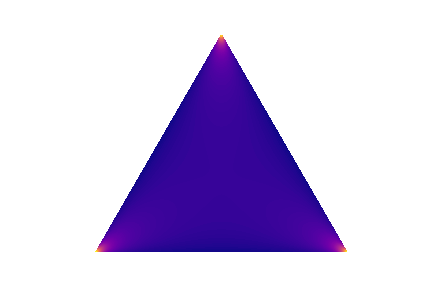
\includegraphics[width=\textwidth]{gs0995.png}
\caption*{$\lambda_\text{temp}=0.995$}
\end{minipage}
\hfill
 \begin{minipage}[t]{.3\textwidth}
   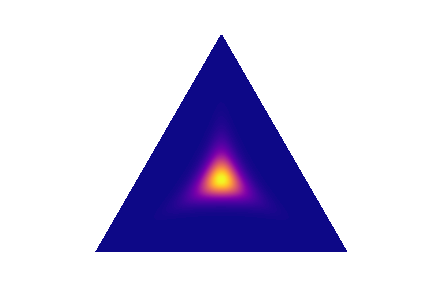
\includegraphics[width=\textwidth]{gs5.png}
\caption*{$\lambda_\text{temp}=5.0$}
\end{minipage}

\end{figure}

\textbf{Dirichlet distribution: }$\textcolor{red}{\boldsymbol{\Gamma}\sim \text{Dir}(\mathbf{s}, \lambda_\text{temp})}$\\
\begin{figure}
 \begin{minipage}[t]{.3\textwidth}
        \centering
\begin{tikzpicture}[%
x={(1.7cm,0cm)},
y={(0cm,1.7cm)},
]

\coordinate (A) at (0,0); 
\coordinate (B) at (1,0) ;
\coordinate (C) at (0.5,0.86); 

%Ecken
\node[circle,scale=0.5,fill=black,draw=black](Ap) at (0,0){};
\node[circle,scale=0.5,fill=black,draw=black](Bp) at (1,0){};
\node[circle,scale=0.5,fill=black,draw=black](Cp) at (0.5,0.86){};

%Kanten
\draw[] (A)
-- (B)  node[midway, below]{}
-- (C)      node[midway, right]{}
-- (A)  node[midway, left]{};

\end{tikzpicture}
\caption*{$\lambda_\text{temp}\to0$}
\end{minipage}
\hfill
 \begin{minipage}[t]{.3\textwidth}
   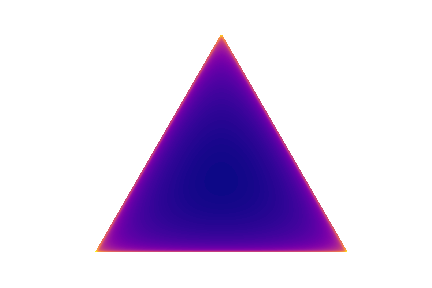
\includegraphics[width=\textwidth]{dir0995.png}
\caption*{$\lambda_\text{temp}=0.995$}
\end{minipage}
\hfill
 \begin{minipage}[t]{.3\textwidth}
   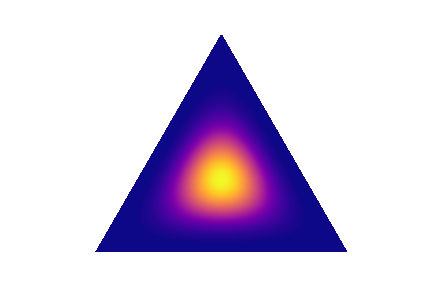
\includegraphics[width=\textwidth]{dir5.png}
\caption*{$\lambda_\text{temp}=5.0$}
\end{minipage}

\end{figure}

\end{frame}


\begin{frame}{Bayesian model selection}


\begin{columns}
\begin{column}{0.4\textwidth}
\textbf{Base model:} %https://www.microsoft.com/en-us/research/wp-content/uploads/2016/02/bishop-variational-icann-98.pdf
\begin{itemize}
\item \textbf{parameters}\\ $\textcolor{red}{\mathbf{w} \sim \mathcal{N}(0, \alpha^{-1})},$
\item \textbf{hyperparameters} $\mathbf{h} = [\alpha].$
\end{itemize}
\begin{figure}
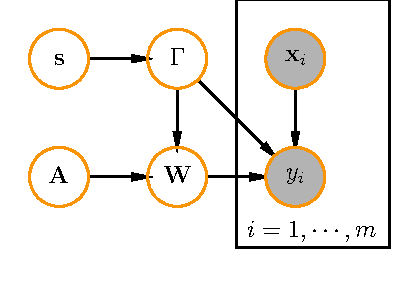
\includegraphics[width=\textwidth]{simple_plate_concrete.pdf}
\end{figure}
\end{column}
\begin{column}{0.6\textwidth}
\textbf{Proposed model: }
\begin{itemize}
\item \textbf{parameters} \\ $\textcolor{red}{\mathbf{w}_r^{j,k} \sim \mathcal{N}(0, (\gamma_{r}^{j,k})^2 (\mathbf{A}_r^{j,k})^{-1})},$
$\mathbf{A}_r^{j,k}$ is a diagonal matrix for the parameters of the primitive function $\mathbf{g}_r^{j,k}$,
\\$\textcolor{OliveGreen}{(\mathbf{A}_r^{j,k})^{-1} \sim \text{inv-gamma}(\lambda_1,\lambda_2)},$

\item \textbf{structure} \\$\boldsymbol{\Gamma} = \{\boldsymbol{\gamma}^{j,k}, (j,k) \in E\},$ \\$\textcolor{red}{\boldsymbol{\gamma}^{j,k} \sim \text{GS}(\mathbf{s}^{j,k}, \lambda_\text{temp})},$ 
\item \textbf{hyperparameters} $\mathbf{h} = [\text{diag}(\mathbf{A}), \mathbf{s} ],$
\item \textbf{metaparameters} $\lambda_1,\lambda_2,\lambda_\text{temp}$.
\end{itemize}

\end{column}

\end{columns}

%

\end{frame}


\begin{frame}{Evidence as a statistical complexity}  
\footnotesize
\textbf{Minimum description length} for the model $\mathbf{f}$:
\[
	\text{MDL}(\mathbf{y},\mathbf{f}) = \textcolor{OliveGreen}{-\text{log}~p(\mathbf{h}|\mathbf{f})} - \textcolor{red}{\text{log}~p(\hat{\mathbf{w}} | \mathbf{h},\mathbf{f})}-  \textcolor{blue}{\text{log}~\bigl(p(\mathbf{y}|\mathbf{X}, \hat{\mathbf{w}},\mathbf{f})\delta\mathfrak{D}\bigr)},
\]
where $\delta\mathfrak{D}$ is an information transmission precision.\\~\\
\textbf{Bayesian approach:}\\
Obtain values of parameters   $\mathbf{w}$ with respect to \textbf{posterior distribution of parameters}:                                      
\[
     L = \text{log} p(\mathbf{w}|\mathbf{X}, \mathbf{y}, \mathbf{h}, \lam) \propto  \textcolor{red}{\text{log} p(\mathbf{y}|\mathbf{X},\mathbf{w}, \mathbf{h},\lam)} +  \textcolor{blue}{\text{log} p(\mathbf{w} |\mathbf{h},\lam)}.
\]

Hyperparameters are optimized using  \textbf{posterior distribution of hyperparameters}:                                      
\[                                                                                                                                              
        Q = \text{log}p(\mathbf{f}|\mathbf{X}, \mathbf{y}) \propto \textcolor{OliveGreen}{\text{log}p(\mathbf{h}|\mathbf{f})} +  \text{log}\int\limits_{\mathbf{w}} \textcolor{red}{p(\mathbf{y}|\mathbf{X},\mathbf{w},\lam)} \textcolor{blue}{p(\mathbf{w}| \mathbf{h},\lam)} d\mathbf{w}.                     
\]       


\begin{figure}
\vspace{-0.5cm}
  \centering    
 \subfloat[]{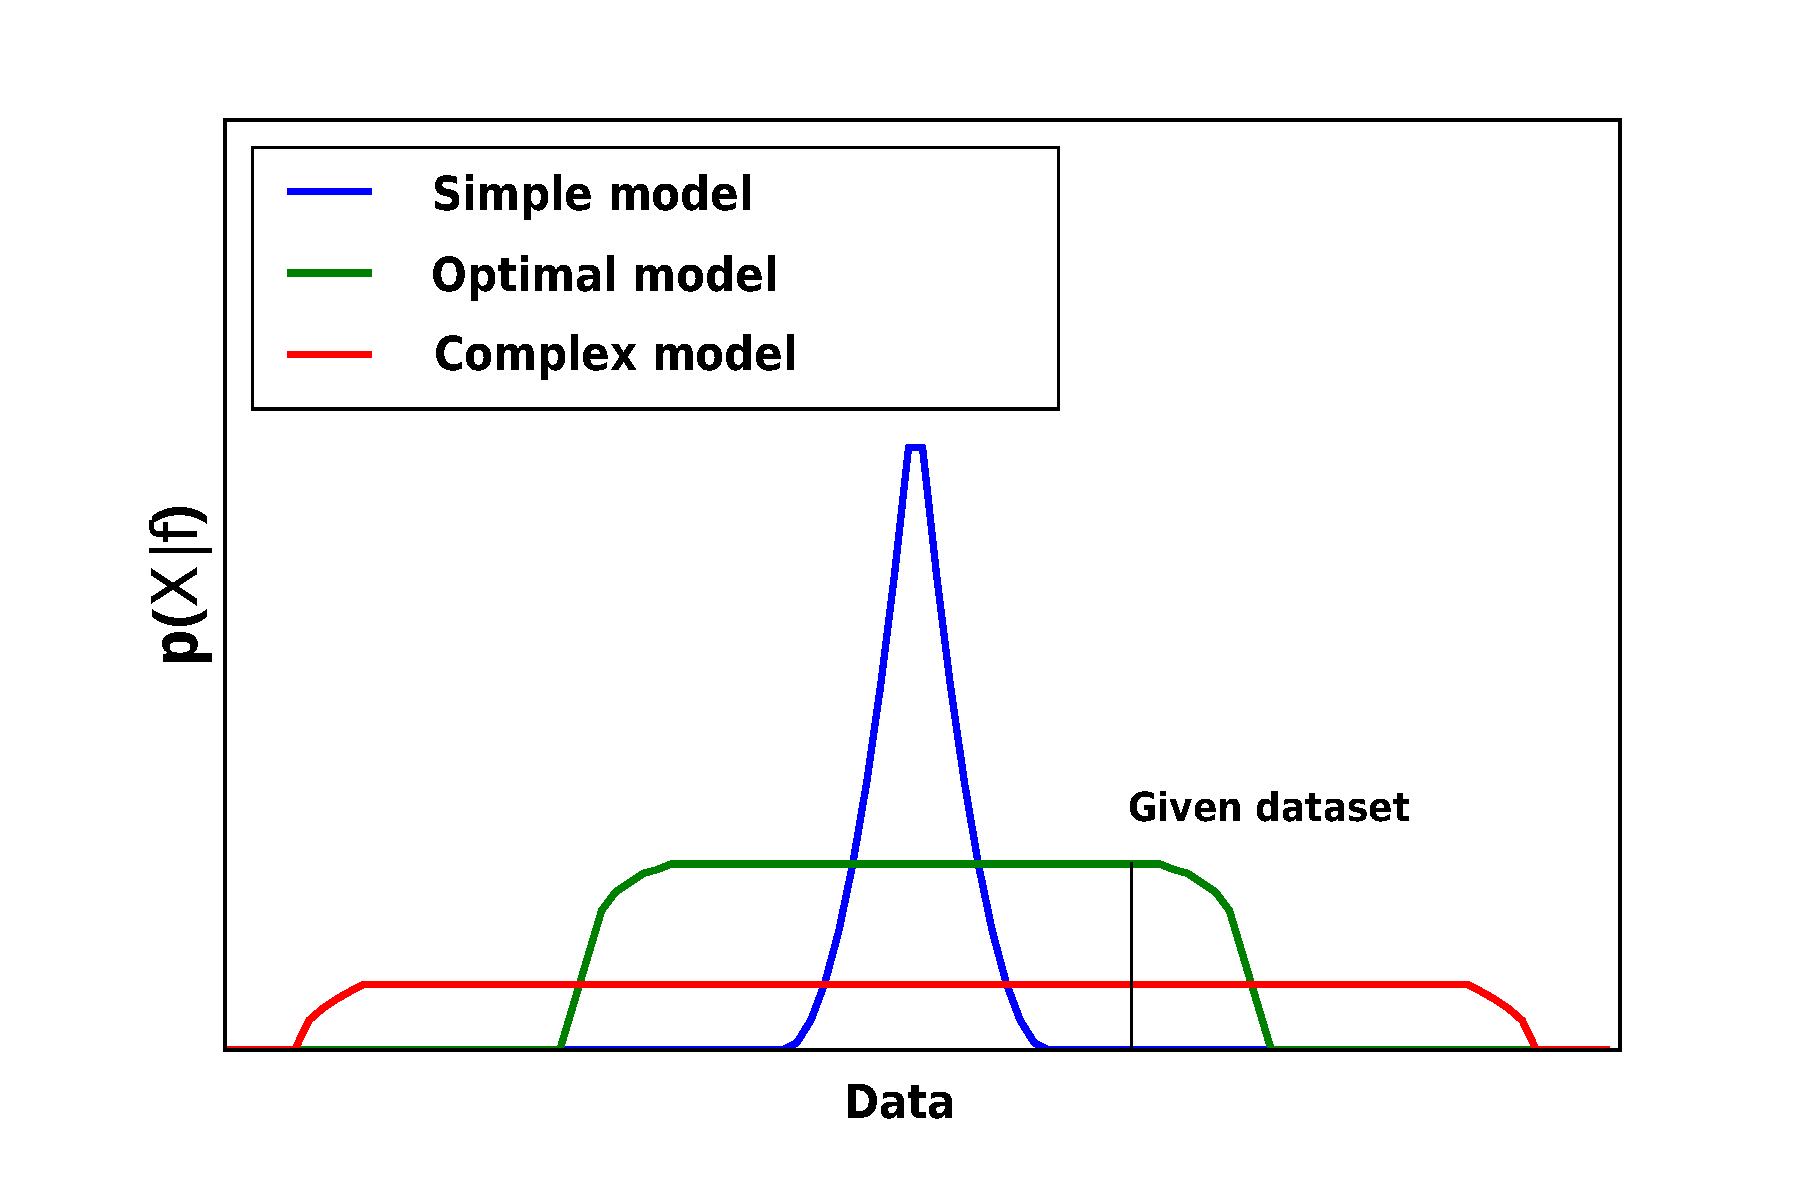
\includegraphics[width=0.43\textwidth]{slide_plots/evidence_en.pdf}} 
 \subfloat[]{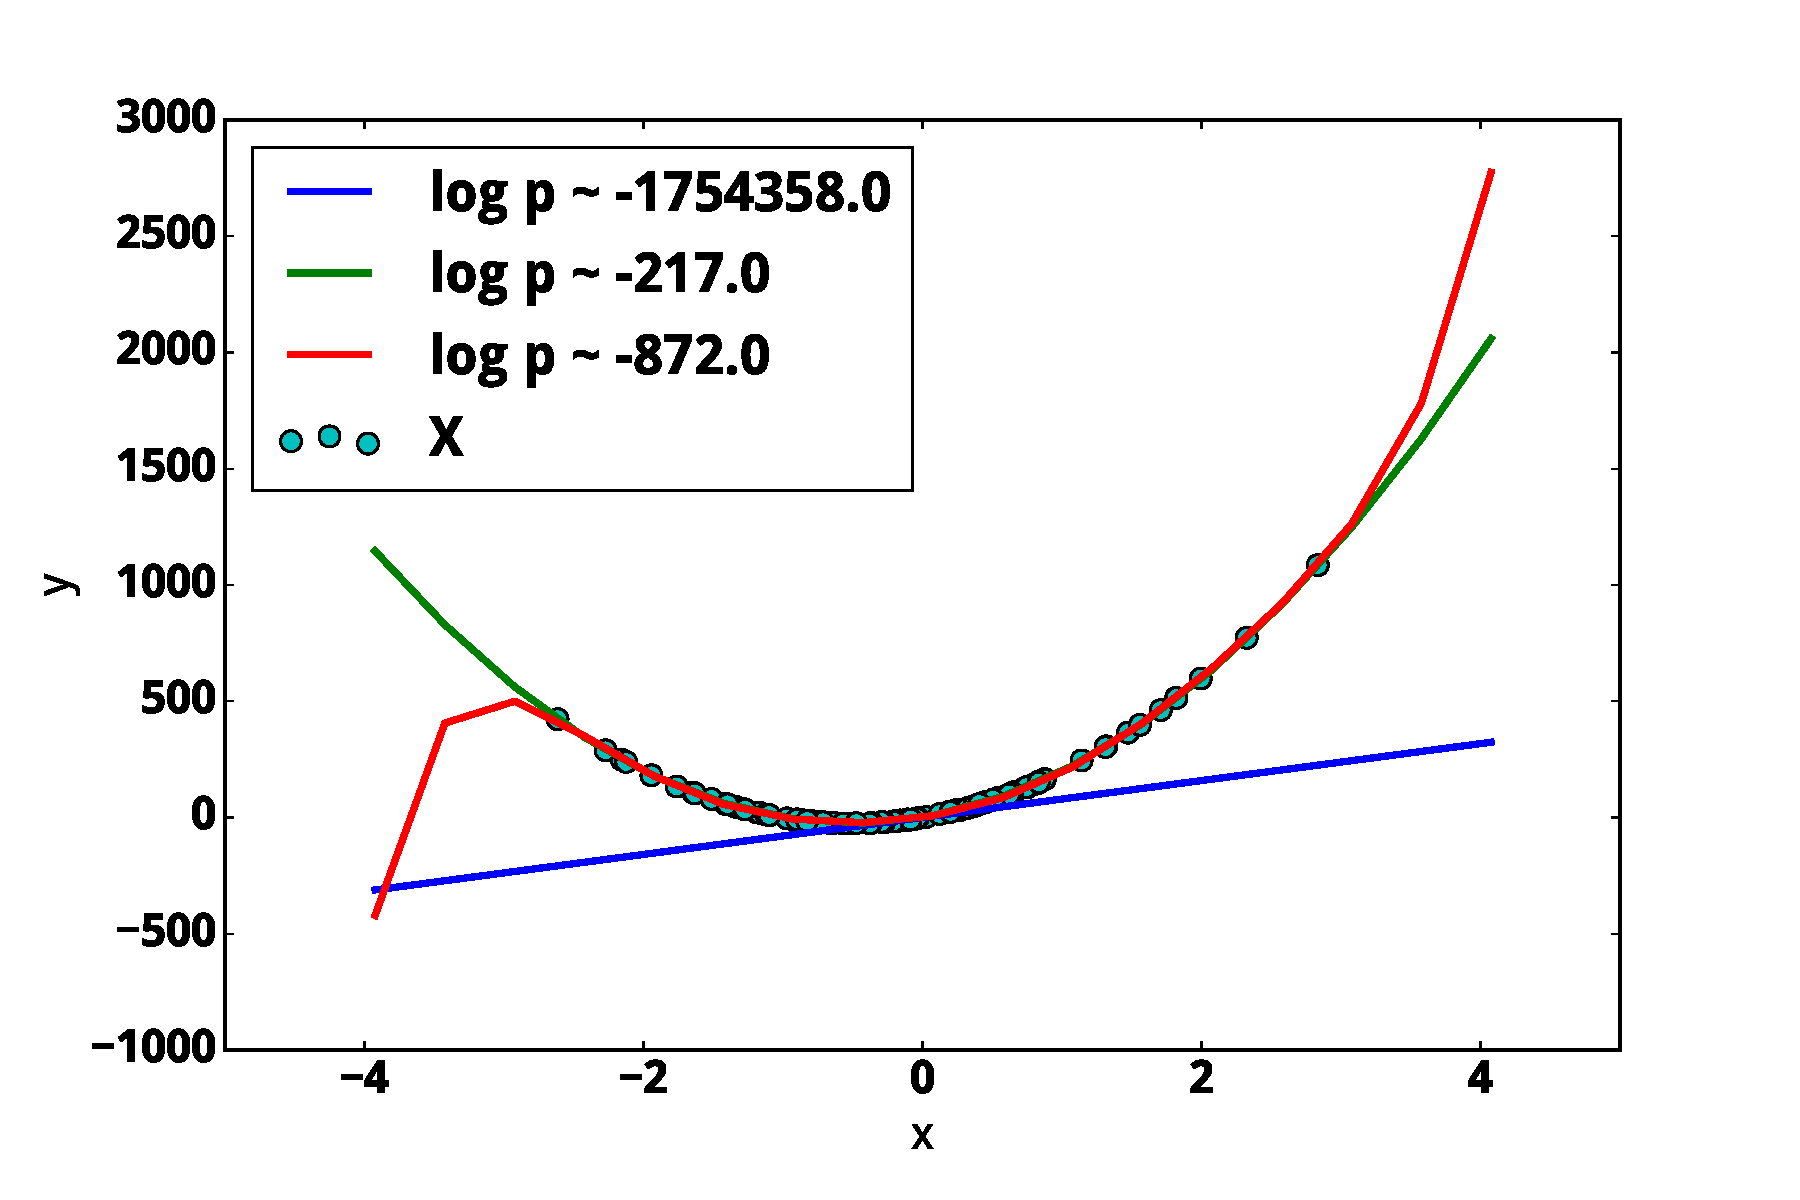
\includegraphics[width=0.43\textwidth]{slide_plots/example.pdf}}

\end{figure}
\end{frame}


\begin{frame}{Evidence lower bound} 
\footnotesize
The evidence is analytically intractable.\\
\textbf{Model evidence:}
\[
p(\mathbf{y}|\mathbf{X}, \h, \lam) =
 \iint\limits_{\mathbf{w}, \boldsymbol{\Gamma}}  \textcolor{red}{p(\mathbf{y}|\mathbf{X},\mathbf{w},  \boldsymbol{\Gamma})} \textcolor{blue}{p(\mathbf{w}, \boldsymbol{\Gamma}|\mathbf{h}, \lam)}d\mathbf{w}d{\boldsymbol{\Gamma}}.                         
\]

\begin{columns}
\begin{column}{0.55\textwidth}
  
\begin{block}{Definition}
\textit{Variational parameters} of the model $\boldsymbol{\theta} \in \Tetab$ are the parameters of the distribution $q$ that approximates posterior distribution $p(\mathbf{w}, \boldsymbol{\Gamma}|\mathbf{X}, \mathbf{y}, \mathbf{h}, \lam)$:
\[
    q \approx  \frac{\textcolor{blue}{p(\mathbf{y}|\mathbf{X},\mathbf{w},\boldsymbol{\Gamma})}\textcolor{red}{p(\mathbf{w}, \boldsymbol{\Gamma}|\mathbf{h}, \lam)}}{\iint\limits_{\mathbf{w}', \boldsymbol{\Gamma'}}\textcolor{blue}{p(\mathbf{y}|\mathbf{X},\mathbf{w}',\boldsymbol{\Gamma}')}\textcolor{red}{p(\mathbf{w}', \boldsymbol{\Gamma}'|\mathbf{h}, \lam)}d\mathbf{w}'d\boldsymbol{\Gamma}'}.
\]
\end{block} 

\end{column}
\begin{column}{0.45\textwidth}  %%<--- here
    \begin{center}
     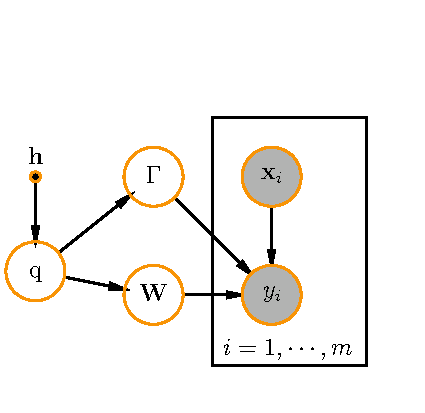
\includegraphics[width=\textwidth]{plate.pdf}
     \end{center}
\end{column}
\end{columns}



%Пусть $q(\mathbf{W}, \boldsymbol{\Gamma}) = q_{\mathbf{W}}(\mathbf{W})q_{\boldsymbol{\Gamma}}(\boldsymbol{\Gamma})$ --- непрерывное распределение, аппроксимирующее 
%апостериорное распределение $p(\mathbf{W}, \boldsymbol{\Gamma}|\mathbf{y}, \mathbf{X})$.
~\\Lower bound of $\text{log}{{p}}(\mathbf{y}|\mathbf{X}, \h, \lam)$:
$$                                                                                                                                              
        \text{log}~p(\mathbf{y}|\mathbf{X}, \h, \lam) \geq 
\textcolor{blue}{\mathsf{E}_q \text{log}~{p(\mathbf{y} | \mathbf{X}, \mathbf{w}, \boldsymbol{\Gamma})}} - \textcolor{red}{\text{D}_{KL}\bigl(q(\mathbf{w}, \boldsymbol{\Gamma})||p(\mathbf{w}, \boldsymbol{\Gamma}| \mathbf{h}, \lam)\bigr)}.
$$ 



The lower bound equals to evidence when $$D_\text{KL}\bigl(q(\mathbf{w}, \boldsymbol{\Gamma})|p\left(\mathbf{w}, \boldsymbol{\Gamma}|\mathbf{y}, \mathbf{X}, \h, \lam\right)\bigr)=0.$$

\end{frame}      


\begin{frame}{Model selection problem}
\footnotesize
Define a variational distribution $q=q_\mathbf{w}q_{\boldsymbol{\Gamma}}$ with parameters $\boldsymbol{\theta}$ that approximates posterior distribution $p(\mathbf{w}, \boldsymbol{\Gamma}|\mathbf{X}, \mathbf{y}, \mathbf{h}, \mathbf{f})$.



\begin{block}{Definition}

\textit{Loss function} $\Loss$ is a differentiable function interpreted as a performance of the model on the train dataset.~\\~\\
\textit{Validation function} $\Val$  is a differentiable function  interpreted as a general performance of the model.
\end{block}
\begin{block}{}
The \textit{model selection problem} $\mathbf{f}$ is a level optimization:

\[
	\mathbf{h}^{*} = \argmax_{\mathbf{h} \in \mathbb{H}} \Val[][][][\teta^{*}],
\]
where $\boldsymbol{\theta}^{*}$ is a solution for the following optimization:
\[
   \boldsymbol{\theta}^{*} = \argmax_{\boldsymbol{\theta} \in \mathbb{U}} \Loss.
\]
\end{block}


\end{frame}







                                                                                                              


   
\begin{frame}{Generalizing optimization problem}
\footnotesize
%\begin{block}{Определение}
The model selection problem  $\mathbf{h}^{*}, \boldsymbol{\theta}^{*}$ is a generalizing problem on the compact $U_{\theta}\times U_{h} \times U_{\lambda} \subset \mathbb{R}^{u} \times \mathbb{H} \times \amsmathbb{\Lambda}$, if the following conditions are met:
\begin{enumerate}
\item For each parameter, hyperparameter and metaparameters its domain is not empty and not a point.
\item For each  $\mathbf{h} \in U_h$ and each  $\boldsymbol{\lambda} \in U_{\lambda}$ the solution  $\boldsymbol{\theta}^{*}$ is uniquely defined.


\item \textbf{Continuance:} $L,Q$ are continuous with respect to metaparameters.
\item \textbf{\textcolor{OliveGreen}{optimal structure exhaustive search: }}
%\textcolor{darkgray}{
there is a constant $K_3>0$  and a value for the  metaparameters $\boldsymbol{\lambda}$ such that for all pairs of local optima $\mathbf{h}_1,\mathbf{h}_2$ of $Q$ with metaparameters $\boldsymbol{\lambda}$ such that  $$D_\text{KL}\left(p(\boldsymbol{\Gamma}| \mathbf{h}_1, \boldsymbol{\lambda}) | p(\boldsymbol{\Gamma}| \mathbf{h}_1, \boldsymbol{\lambda})\right) > K_3, D_\text{KL}\left(p(\boldsymbol{\Gamma}| \mathbf{h}_1, \boldsymbol{\lambda}) | p(\boldsymbol{\Gamma}| \mathbf{h}_2, \boldsymbol{\lambda})\right) > K_3,$$ $$Q(\mathbf{h}_1|\boldsymbol{\lambda})>Q(\mathbf{h}_2|\boldsymbol{\lambda}),$$  there exists another value of metaparameters $\boldsymbol{\lambda}' \neq \boldsymbol{\lambda}$ that
\begin{enumerate}
\item the  correspondence between optimal variational parameters and hyperparameters  $\boldsymbol{\theta}^{*}(\mathbf{h}_1),\boldsymbol{\theta}^{*}(\mathbf{h}_2)$ remains for $\boldsymbol{\lambda}'$,
\item the following inequality is satisfied: $Q(\mathbf{h}_1|\boldsymbol{\lambda}')<Q(\mathbf{h}_2|\boldsymbol{\lambda}')$.
\end{enumerate}
%}



\end{enumerate}
%\end{block}
\end{frame}

\begin{frame}{Generalizing optimization problem}
\footnotesize
%\begin{block}{Определение}
The model selection problem  $\mathbf{h}^{*}, \boldsymbol{\theta}^{*}$ is generalizing on the compact $U_{\theta}\times U_{h} \times U_{\lambda} \subset \mathbb{R}^{u} \times \mathbb{H} \times \amsmathbb{\Lambda}$, if the following conditions are met:
\begin{enumerate}
\setcounter{enumi}{4}
\item \textbf{ \textcolor{blue}{Likelihood maximization: }}\textcolor{darkgray}{ there is a metaparameter value $\boldsymbol{\lambda} \in U_{\lambda}$ and  $K_1 \in \mathbb{R}_{+}$ such that for each pair of hyperparameter vectors $\mathbf{h}_1, \mathbf{h}_2 \in  U_{h}, Q(\mathbf{h}_1) - Q(\mathbf{h}_2) > K_1$ the following inequality is satisfied : $\mathsf{E}_q \text{log}~p(\mathbf{y}|\mathbf{X}, \boldsymbol{\theta}^{*}(\mathbf{h}_1), \lambda_{\text{temp}}, \mathbf{f})>\text{log}\mathsf{E}_q ~p(\mathbf{y}|\mathbf{X}, \boldsymbol{\theta}^{*}(\mathbf{h}_2), \lambda_{\text{temp}}, \mathbf{f})$.}

% здесь мы имеем ввиду что для любого lambda, такого что мы считаем параметр неинформативными
\item \textbf{\textcolor{red}{Сomplexity minimization: }}\textcolor{darkgray}{ there is a metaparameter value  $\boldsymbol{\lambda} \in U_{\lambda}$ and $K_2 \in \mathbb{R}_{+}$ such that for each pair of hyperparameter vectors $\mathbf{h}_1, \mathbf{h}_2 \in U_h, Q(\mathbf{h}_1) - Q(\mathbf{h}_2) > K_2$,  $\mathsf{E}_q \text{log}~p(\mathbf{y}|\boldsymbol{\theta}_1, \lambda_{\text{temp}}, \mathbf{f}) = \text{log}\mathsf{E}_q ~p(\mathbf{y}|\boldsymbol{\theta}_2, \lambda_{\text{temp}}, \mathbf{f})$, the complexity of the first model is less than the second one.}

\item \textbf{Evidence lower bound optimization: }\textcolor{darkgray}{ there is a metaparameter value  $\boldsymbol{\lambda}$, such that the optimization is equivalent to the evidence lower bound optimization:
\vspace{-0.2cm}
\[
    \mathbf{h}^{*} \propto \argmax_{} \log \E_{\q} \LL - \KL{\q}{\prior} + \log p(\mathbf{h}|\boldsymbol{\lambda}),
\]
\[
    \boldsymbol{\theta}^{*} = \argmin D_\text{KL}(q| p(\mathbf{w}, \boldsymbol{\Gamma}|\mathbf{y}, \mathbf{X}, \h, \lam)).
\]}
\vspace{-0.6cm}
\end{enumerate}
%\end{block}
\end{frame}

\begin{frame}{Model selection problem analysis}
\small
\begin{block}{Theorem [Bakhteev, 2019]}
The following problems are not generalizing:
\begin{enumerate}
% задача не является строго двууровневой, нельзя проомтимизировать ELBO
\item maximum likelihood criterion: $\max_{\boldsymbol{\theta}} \textcolor{blue}{\mathsf{E}_q \text{log} p(\mathbf{y}|\mathbf{X}, \boldsymbol{\theta}, \h, \lam)};$

% нет возможности оптимизации структуры
\item maximum posterior probability criterion: $\max_{\boldsymbol{\theta}} \textcolor{blue}{\mathsf{E}_q \text{log} p(\mathbf{y}|\mathbf{X},  \boldsymbol{\theta}, \mathbf{f})}\textcolor{red}{p( \boldsymbol{\theta}| \mathbf{h}, \lam)};$

% нет возможности оптимизации правдоподобия модели - структа не подчиняется beta
\item evidence lower bound maximization: $\max_{\mathbf{h}} \max_{\boldsymbol{\theta}} \textcolor{blue}{\mathsf{E}_q \text{log} \LL} - \textcolor{red}{\KL{\prior}{\q}\bigr)}  + \textcolor{OliveGreen}{ \text{log} p(\mathbf{h}|\mathbf{f})};$

\item cross-validation: $\max_{\mathbf{h}} \textcolor{blue}{\mathsf{E}_q \text{log}p(\mathbf{y}_\text{valid}|\mathbf{X}_\text{valid}, \boldsymbol{\theta}^{*})}$, $\boldsymbol{\theta}^{*} = \argmax_{\boldsymbol{\theta}} \textcolor{blue}{\mathsf{E}_q \text{log}p(\mathbf{y}_\text{train}|\mathbf{X}_\text{train}, \h, \lam)} \textcolor{red}{p(\boldsymbol{\theta}| \mathbf{h})}$.

% задача не является строго двууровневой, нельзя проомтимизировать ELBO
\item AIC: $\max_{\boldsymbol{\theta}} \textcolor{blue}{\mathsf{E}_q \text{log} p(\mathbf{y}|\mathbf{X}, \boldsymbol{\theta}, \lambda_\text{temp}, \mathbf{f})} - \textcolor{red}{|\theta_i: \text{D}_\text{KL}\left(q(w_i)|p(w_i|\boldsymbol{\Gamma}, \mathbf{h}, \boldsymbol{\lambda}\right) < \lambda|}$;

% задача не является строго двууровневой, нельзя проомтимизировать ELBO
\item BIC: $\max_{\boldsymbol{\theta}} \textcolor{blue}{\mathsf{E}_q \text{log} p(\mathbf{y}|\mathbf{X}, \boldsymbol{\theta}, \lambda_\text{temp}, \mathbf{f})} - \textcolor{red}{\frac{1}{2}\text{log}(|\mathbb{W}|{|\theta_i: \text{D}_\text{KL}\left(q(w_i)|p(w_i|\boldsymbol{\Gamma}, \mathbf{h}, \boldsymbol{\lambda}\right) < \lambda|}}$;


\item structure exhaustive search:  $\max{\boldsymbol{\Gamma}'} \max_{\boldsymbol{\theta}} \textcolor{blue}{\mathsf{E}_q \text{log} p(\mathbf{y}|\mathbf{X}, \boldsymbol{\theta}, \lambda_\text{temp}, \mathbf{f})}\textcolor{red}{\mathbb{I}(q(\boldsymbol{\Gamma}{\Gamma} = p') },$ where $p'$ is a distribution on a structure (metaparameter).
\end{enumerate}
\end{block}
\end{frame}

\begin{frame}{Proposed optimization problem}

\footnotesize
\begin{columns}
\begin{column}{0.8\textwidth}
\begin{block}{Theorem [Bakhtreev, 2019]}
The following problem is generalizing:
\[
\mathbf{h}^{*} = \argmax_{\mathbf{h}} Q = 
\]
\[
= \textcolor{blue}{\lamLL\mathsf{E}_{\q[\teta^{*}]} \text{log}~{p(\mathbf{y} | \mathbf{X}, \mathbf{w},\boldsymbol{\Gamma}, \mathbf{h}, \lam)}}
 -\]
\vspace{-0.3cm}
\[- \textcolor{red}{^\text{prior}_\text{Q}\text{D}_{KL}\bigl(\q[\teta^{*}] || p(\mathbf{w}, \boldsymbol{\Gamma} |\mathbf{h}, \lam) \bigr)}  -\]
\vspace{-0.3cm}
\[
 - \textcolor{OliveGreen}{\sum_{p' \in \mathfrak{P}, \lambda \in \boldsymbol{\lambda}^\text{struct}_\text{Q}} \lambda\text{D}_{KL}(\priorG | p') + \text{log}p(\mathbf{h}|\lam)}, 
\]
where 
\[
\teta^{*} = \argmax_{\teta} L = 
\textcolor{blue}{\mathsf{E}_q \text{log}~{p(\mathbf{y} | \mathbf{X}, \mathbf{w}, \boldsymbol{\Gamma}, \mathbf{h}, \lam)}}
\]
\vspace{-0.3cm}
\[- \textcolor{red}{^\text{prior}_\text{L}\text{D}_{KL}\bigl( q^{*}(\mathbf{w}, \boldsymbol{\Gamma}) || p(\mathbf{w}, \boldsymbol{\Gamma} |\mathbf{h}, \lam) \bigr)}.
\]
\end{block}
%$\lambda^\text{likelihood}_\text{L}, \lambda^\text{prior}_\text{L}, \lambda^\text{prior}_\text{Q},  \boldsymbol{\lambda}_{\text{struct}}^Q, \lambda_{\text{temp}}$ и параметры распределений $\mathbf{P}$ --- метапараметры оптимизации.\\
The proposed optimization generalized different optimization problems: maximum likelihood and evidence lower bound optimization, model complexity increase and decrease, exhaustive structure search.
\end{column}
\begin{column}{0.2\textwidth}
\begin{figure}
\centering
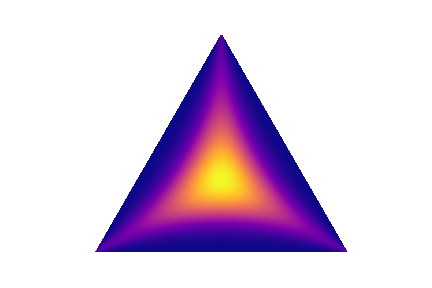
\includegraphics[width=0.75\textwidth]{combinations_1.png}
\end{figure}
\vspace{-0.2cm}
$ \textcolor{OliveGreen}{\boldsymbol{\lambda}_{\text{struct}}^Q=[0;0;0].}$
\begin{figure}
\centering
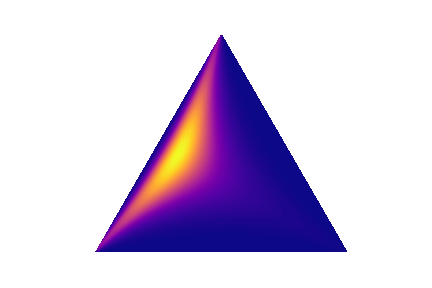
\includegraphics[width=0.75\textwidth]{combinations_2.png}
\end{figure}
\vspace{-0.2cm}
$ \textcolor{OliveGreen}{\boldsymbol{\lambda}_{\text{struct}}^Q=[1;0;0].}$
\begin{figure}
\centering
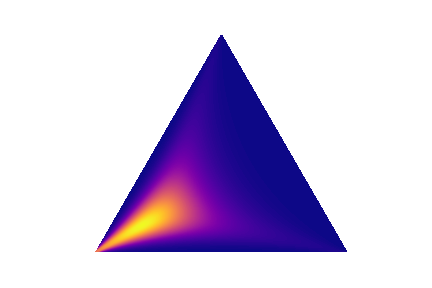
\includegraphics[width=0.75\textwidth]{combinations_3.png}
\end{figure}
\vspace{-0.2cm}
$ \textcolor{OliveGreen}{\boldsymbol{\lambda}_{\text{struct}}^Q=[1;1;0].}$
\end{column}
\end{columns}
\end{frame}


\begin{frame}{Bayesian interpretation of the proposed optimization}
\footnotesize
\begin{block}{Theorem, [Bakhteev, 2018]}
Define a set of variational distribution $q(\boldsymbol{\theta})$. 

Let $\textcolor{blue}{\lambda^L_\text{likelihood}} = \textcolor{red}{\lambda^L_\text{prior}=\lambda^Q_\text{prior}}=1, \textcolor{OliveGreen}{\boldsymbol{\lambda}^Q_{\text{struct}}}=\mathbf{0}$. Then:
\begin{enumerate}
\item Solution of the proposed optimization problem obtains a maximum posterior distribution for the hyperparameters with evidence lower bound approximation:
\vspace{-0.3cm}
\[
    \text{log}\hat{p}(\mathbf{y}|\mathbf{X}, \mathbf{h}, \lambda_\text{temp}, \mathbf{f}) + \textcolor{OliveGreen}{\text{log}p(\mathbf{h}|\mathbf{f})} \to \max_{\mathbf{h}}.
\]
\item Variational distribution $q$ for the solution approximates posterior distribution  $p(\mathbf{w}, \boldsymbol{\Gamma}|\mathbf{y}, \mathbf{X}, \mathbf{h}, \lambda_\text{temp}, \mathbf{f})$ in the best way:
\vspace{-0.3cm}
\[
    {D}_\text{KL}(q||p(\mathbf{w}, \boldsymbol{\Gamma}|\mathbf{y}, \mathbf{X}, \mathbf{h}, \lambda_\text{temp}, \mathbf{f})) \to \min_{\boldsymbol{\theta}}.
\]
\end{enumerate}
\end{block}
% proof
% 1. по определению
% 2. тоже по определению
\begin{block}{}
Let $q$ be decomposed into two distributions for parameters $\mathbf{w}$ and structure $\boldsymbol{\Gamma}$ of the model $\mathbf{f}$:
\[
    q = q_{\mathbf{w}}q_{\boldsymbol{\Gamma}}, q_{\boldsymbol{\Gamma}} \approx p(\boldsymbol{\Gamma}|\mathbf{y}, \mathbf{X}, \mathbf{h}, \mathbf{f}), q_{\mathbf{w}} \approx p(\mathbf{w}|\boldsymbol{\Gamma},\mathbf{y}, \mathbf{X}, \mathbf{h}, \mathbf{f}).
\]
If there are values for the variational parameters such that $q(\mathbf{w}) = p(\mathbf{w}| \boldsymbol{\Gamma}, \mathbf{h}, \boldsymbol{\lambda}),$ $q(\boldsymbol{\Gamma}) = p(\boldsymbol{\Gamma}| \mathbf{h}, \boldsymbol{\lambda}),$
then the solution of optimization of $L$ is equal to these values.
\end{block}
%http://akosiorek.github.io/ml/2017/09/10/kl-hierarchical-vae.html. Важно: D_KL во втором случае - условная
% декомпозируем на два D_KL
% обе D_KL независимы как функции, поэтому ок, можем минимизировать
\end{frame}





\begin{frame}{Optimization operator}
\small
\begin{block}{Definition}
An \textit{optimization operator}  $T$ is an estimation of the new vector of parameters $\boldsymbol{\theta}'$  using the previous one $\boldsymbol{\theta}$.
\end{block}
Stochastic gradient descent operator
:\[
	 \hat{\boldsymbol{\theta}} = T \circ T \circ \dots \circ T(\boldsymbol{\theta}_0, \mathbf{h}) = T^\eta(\boldsymbol{\theta}_0, \mathbf{h}), \quad\text{где}	T(\boldsymbol{\theta}, \mathbf{h}) =
\]
\[=\boldsymbol{\theta} - \lambda_\text{lr} \nabla \left(-L(\boldsymbol{\theta}, \mathbf{h})|_{\hat{\mathfrak{D}}}\right), 
\]
$\lambda_{\text{lr}}$ is a learning rate, $\boldsymbol{\theta}_0$ is an initial state for  $\boldsymbol{\theta}$, $\hat{\mathfrak{D}}$ is a random subsample of the dataset $\mathfrak{D}$.


Reformulate the optimization problem:
\[
	 \mathbf{h}' = T^\eta\bigl(Q, \mathbf{h}, T^\eta(L, \boldsymbol{\theta}_0, \mathbf{h})\bigr).
\]


\begin{block}{Theorem, [Bakhteev, 2019]}
Let $\frac{\lambda^Q_\text{prior}}{\lambda^Q_\text{likelihood}} = {\lambda^L_\text{prior}}.$ Then the proposed optimization is an one-level optimization.
\end{block}

\end{frame}



\begin{frame}{Hyperparameter optimization: example}
The hyperparameter gradient-based optimization methods were investigated.\\

\begin{multicols}{2}

\begin{figure}[h]
\hspace*{-1cm}
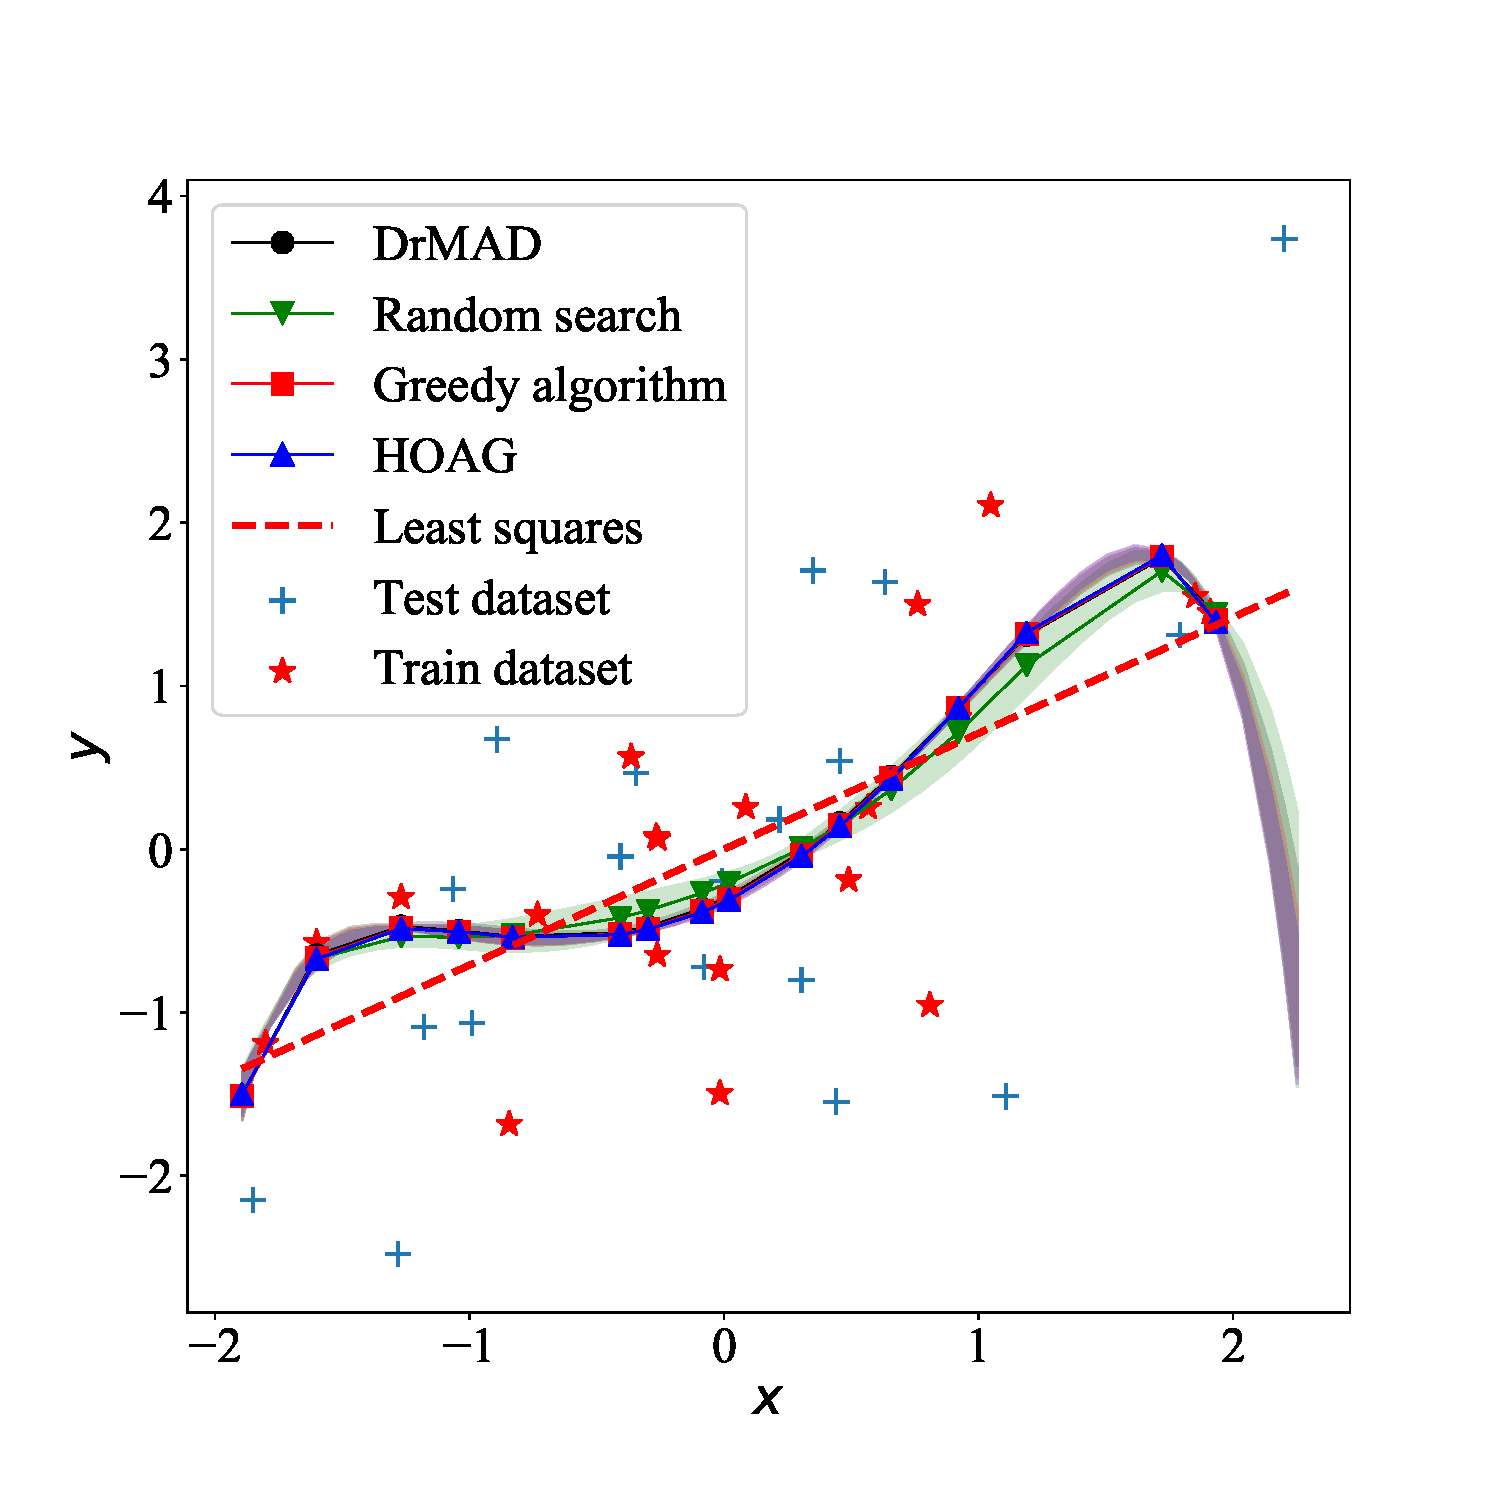
\includegraphics[width=0.5\textwidth]{./slide_plots/Fig_poly_cv2.pdf}
\caption*{Cross-validation}
\end{figure}

\begin{figure}[h]
\hspace*{-1cm}
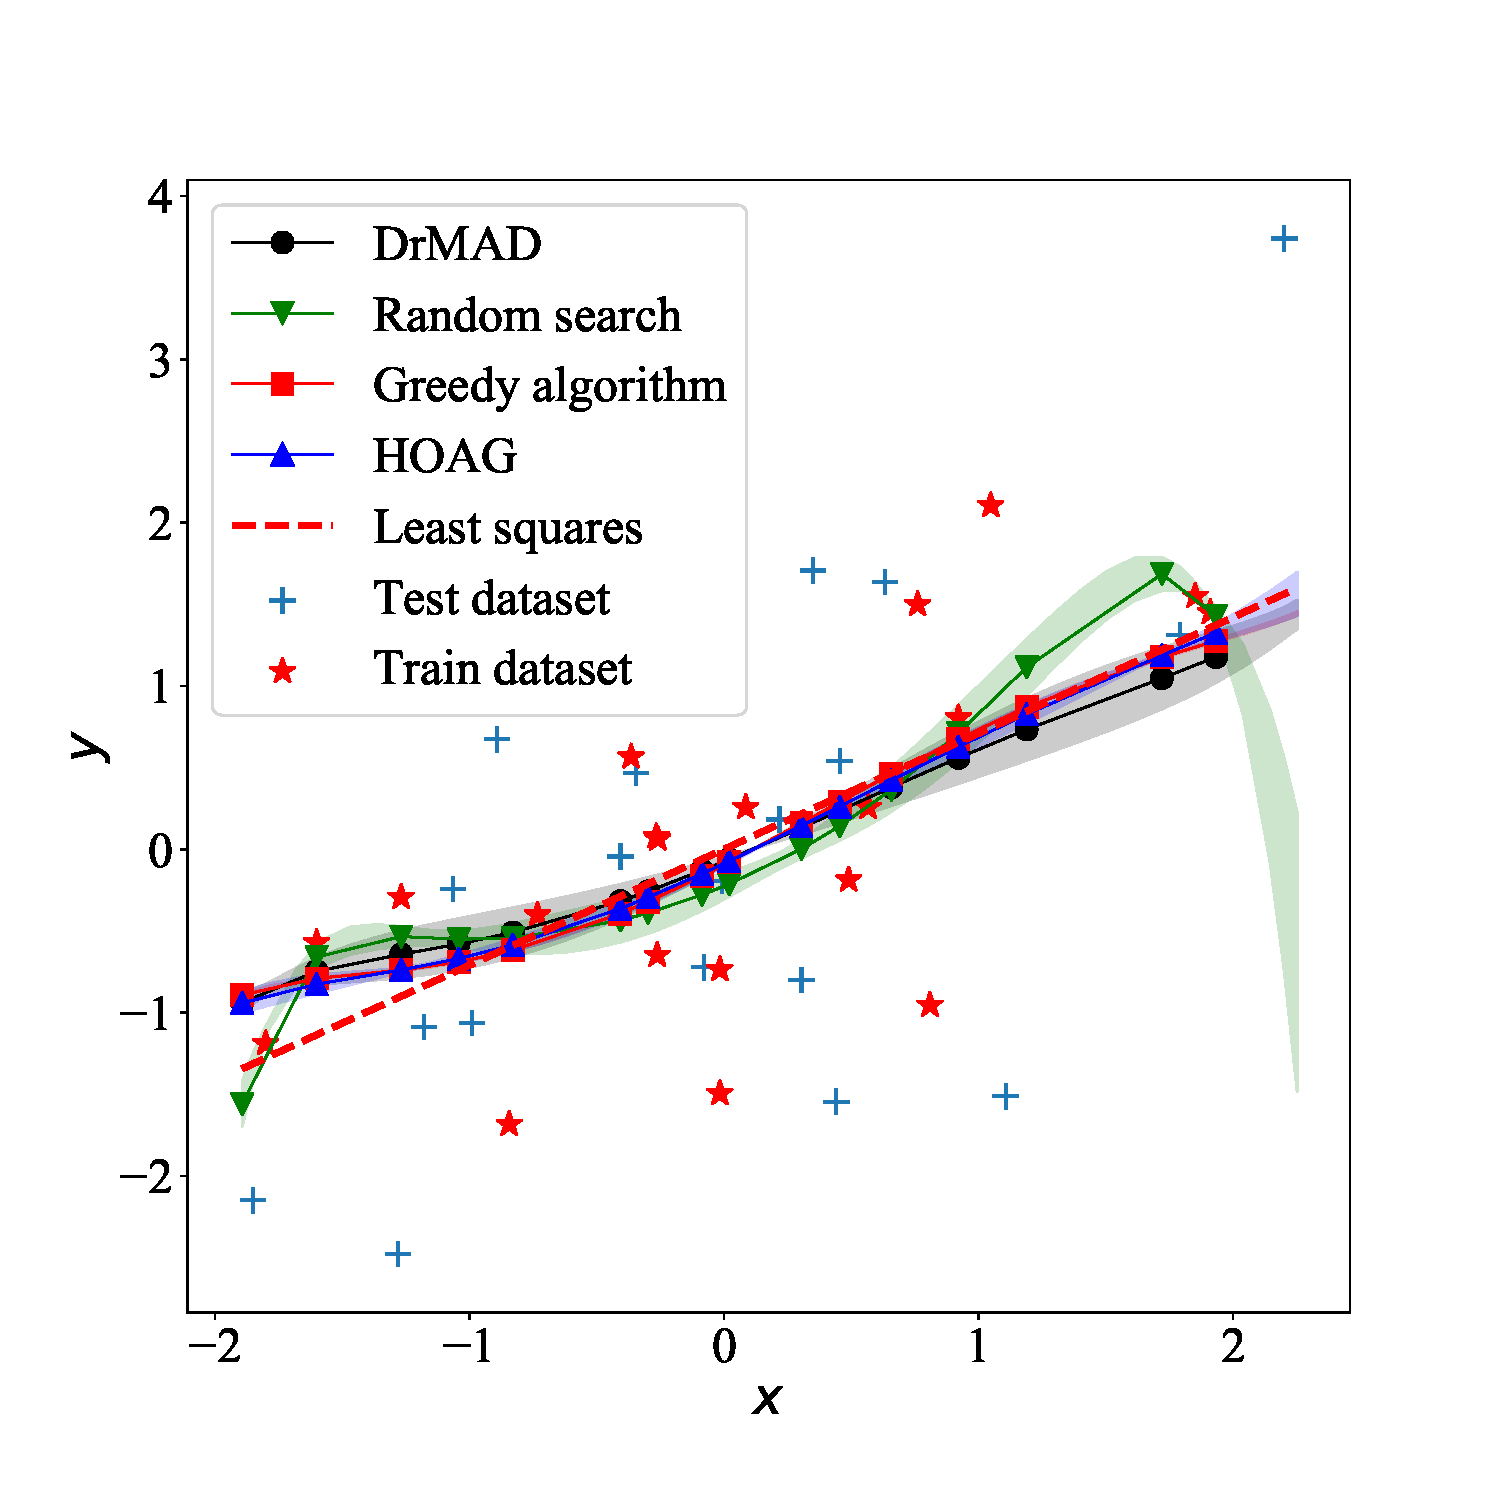
\includegraphics[width=0.5\textwidth]{./slide_plots/Fig_poly_var2.pdf}
\caption*{Evidence lower bound}
\end{figure}
\end{multicols}

\end{frame}



\begin{frame}{Experiments: WISDM}
\begin{figure}  
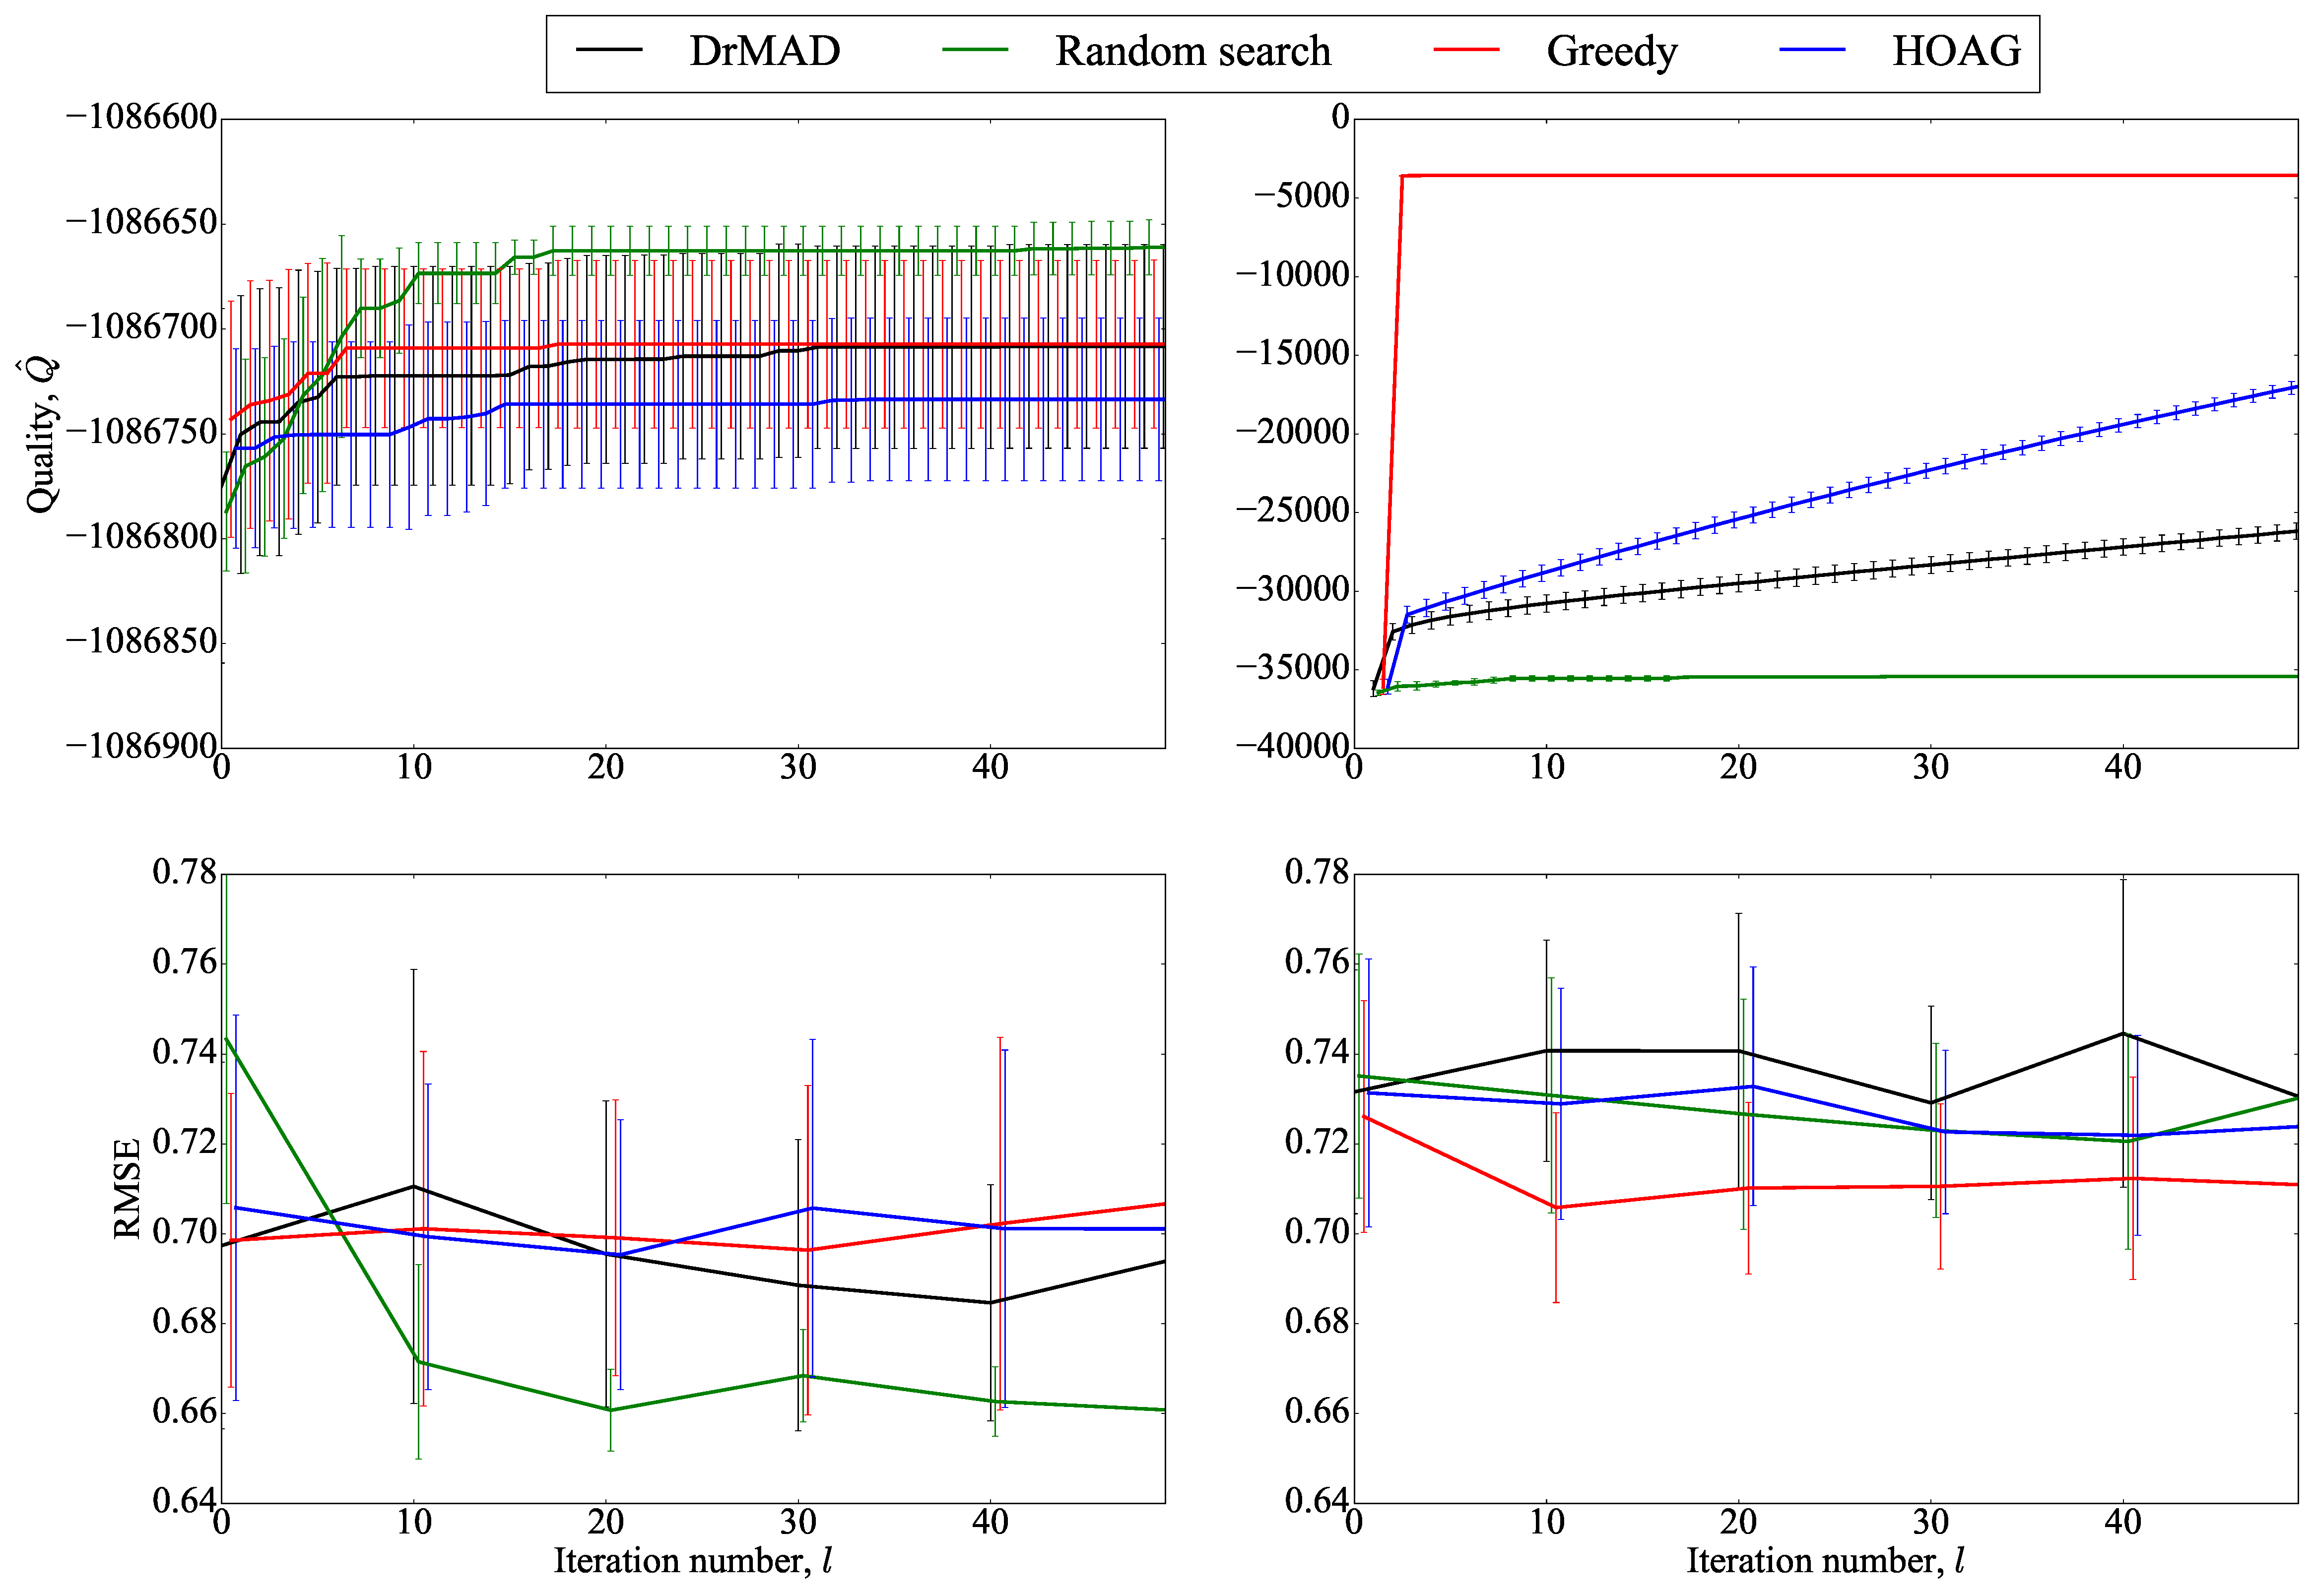
\includegraphics[width=0.85\textwidth]{Fig_wisdm.eps}
\end{figure}
\end{frame}

\begin{frame}{Experiments: MNIST}
\begin{figure}  
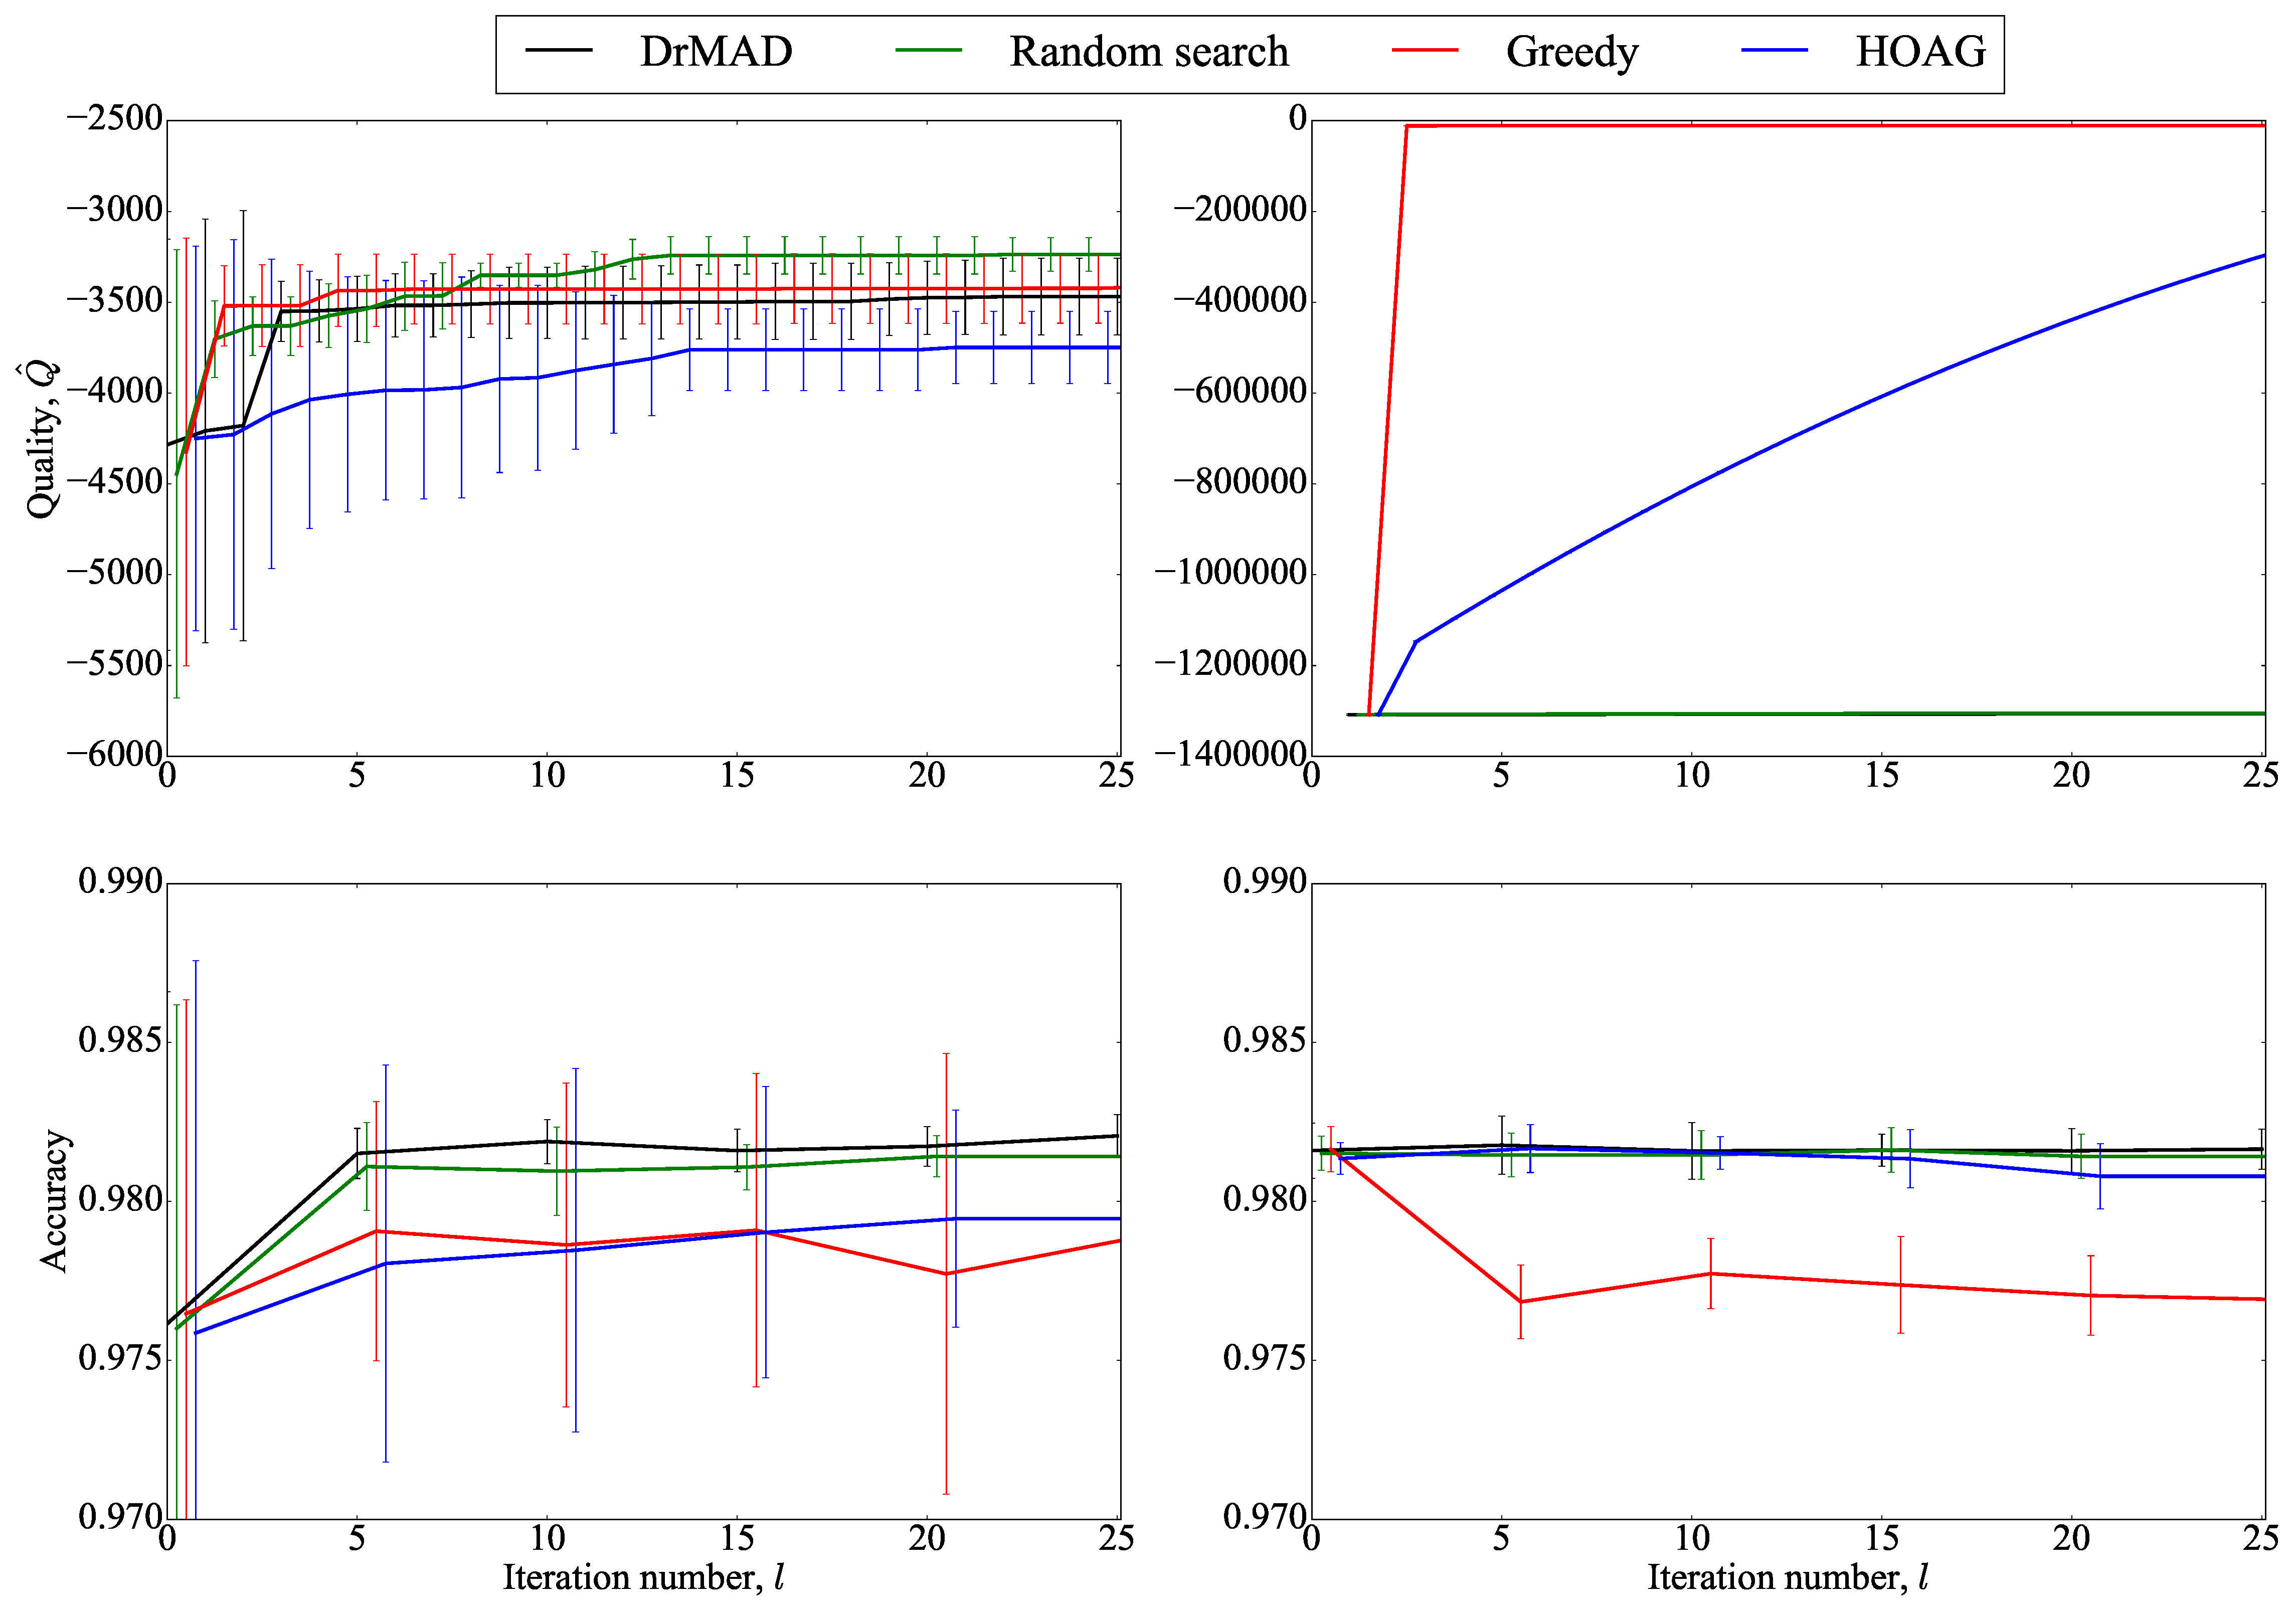
\includegraphics[width=0.85\textwidth]{Fig_mnist.eps}
\end{figure}
\end{frame}


\begin{frame}{Experiments: MNIST}
Noise adjusment $\mathcal{N}(\mathbf{0},\sigma^2\mathbf{I})$:
\setlength{\columnsep}{10pt}
\begin{multicols}{4}
\begin{figure}[h]
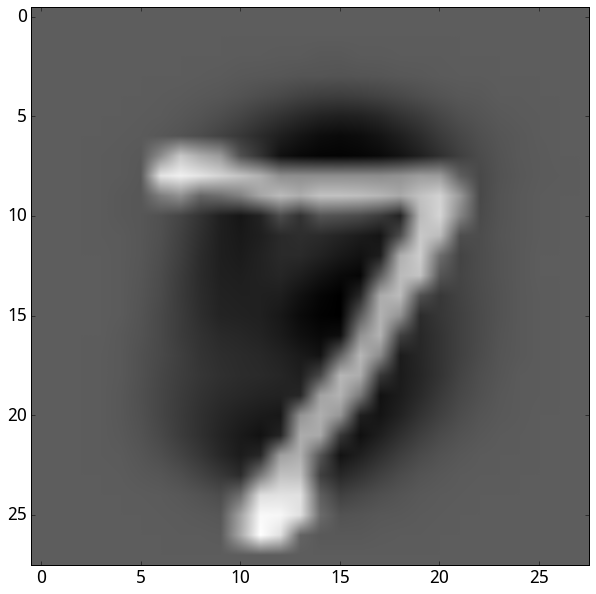
\includegraphics[width=0.10\textwidth]{./mnist0.png}
\caption*{Original images}
\end{figure}

\begin{figure}[h]
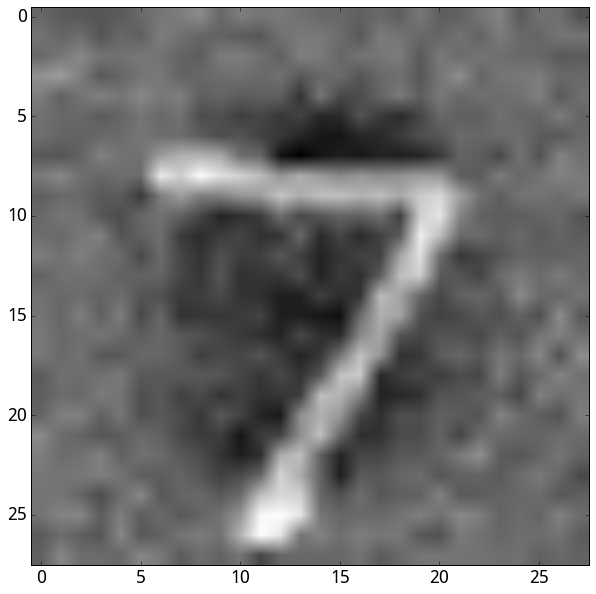
\includegraphics[width=0.08\textwidth]{./mnist10.png}
\caption*{$\sigma=0.1$}
\end{figure}

\begin{figure}[h]
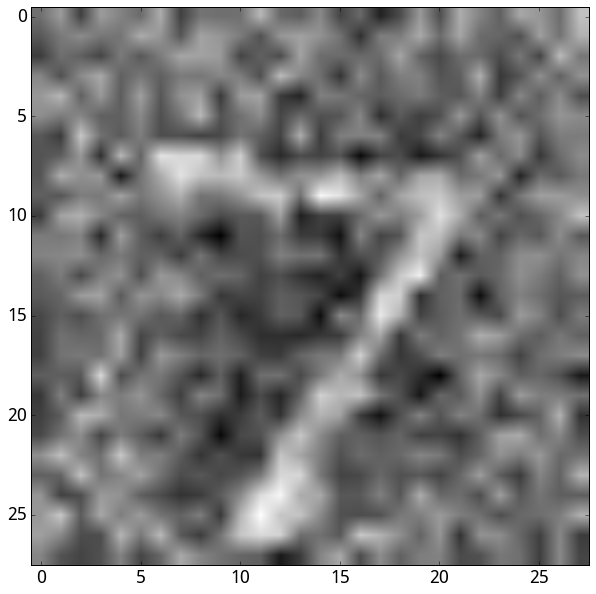
\includegraphics[width=0.08\textwidth]{./mnist25.png}
\caption*{$\sigma=0.25$}
\end{figure}

\begin{figure}[h]
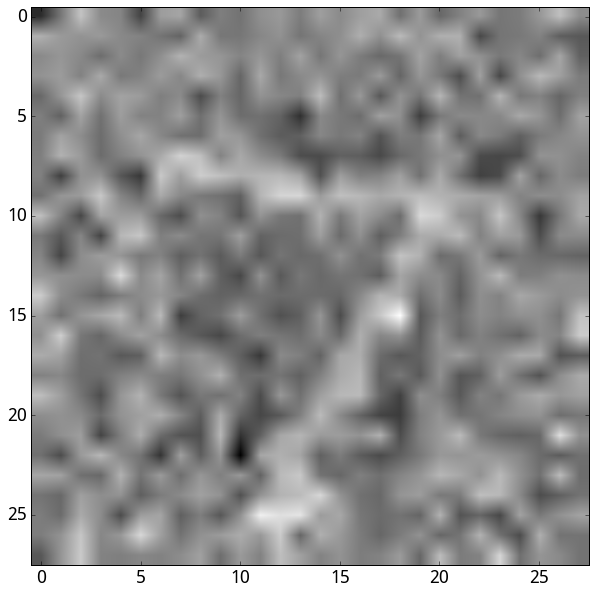
\includegraphics[width=0.08\textwidth]{./mnist50.png}
\caption*{$\sigma=0.5$}
\end{figure}
\end{multicols}
\begin{center}
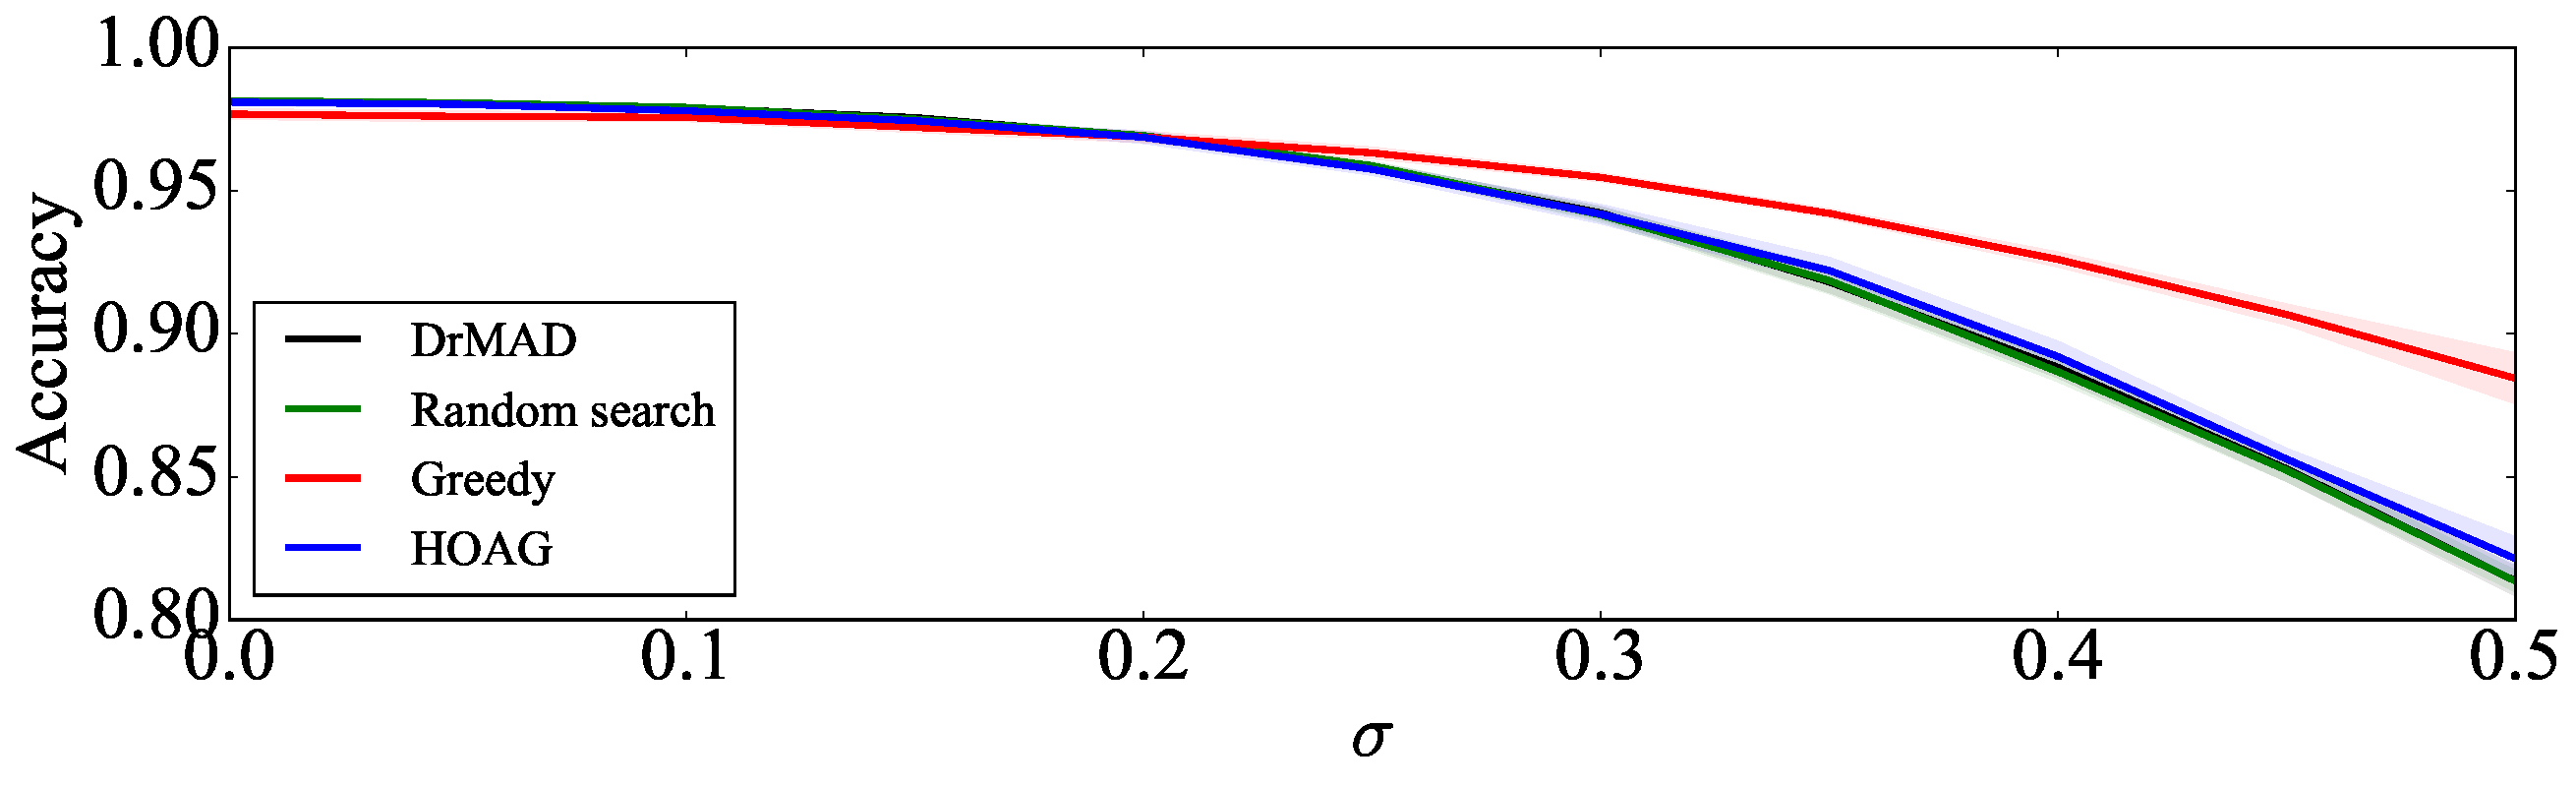
\includegraphics[width=0.85\textwidth]{Fig_noise.pdf}
\end{center}
\end{frame}


\begin{frame}
\small
\frametitle{Evidence lower bound using multi-start}
$$\text{log}p(\mathbf{y}|\mathbf{X}, \mathbf{h},\mathbf{f}) \geq \mathsf{E}_{q(\mathbf{W)}}\text{log~}p (\mathbf{y}, \mathbf{w}|\mathbf{X}, \mathbf{h},\mathbf{f}) - \mathsf{E}_{q_{\mathbf{w}}}(-\text{log}(q_\mathbf{w})).$$

\begin{block}{Theorem [Bakhteev, 2016]} Let  $L$ be a loss function with continuously-differentiable gradient with Lipshitz constant $C$. \\
Let $\boldsymbol{\theta} = [\mathbf{w}^1,\dots,\mathbf{w}^k]$ be a vector of initial states of multiple model optimizations, $\lambda_\text{lr}$ is a learning rate.

Then the difference of differentiable entropies for the optimization step can be estimated:
\small
\[
	\mathsf{E}_{q^{\tau}_{\mathbf{w}}}(-\text{log}(q^{\tau}_\mathbf{w})) -  \mathsf{E}_{q^{\tau-1}_{\mathbf{w}}}(-\text{log}(q^{\tau-1}_\mathbf{w}))  \approx  \frac{1}{k}\sum_{r=1}^k \bigl(\lambda_\text{lr} Tr[\mathbf{H}(\mathbf{w}^r)] - \lambda_\text{lr}^2 Tr[\mathbf{H}(\mathbf{w}^r)\mathbf{H}(\mathbf{w}^r)]  \bigr),
\]
where $\mathbf{H}$ is a Hessian of the negative loss function $-L$, $q^{\tau}_\mathbf{w}$ is a distribution $q$ at the iteration $\tau$.
\end{block}
\end{frame}



\begin{frame}

\frametitle{Gradient descent as an evidence lower bound}
\footnotesize
Empirical distribtuion of the optimized model parameters is a variational distribution.\\


\begin{multicols}{2}
Gradient descent does not optimize evidence lower bound.
\vspace{-1.cm}
\begin{figure}

\subfloat{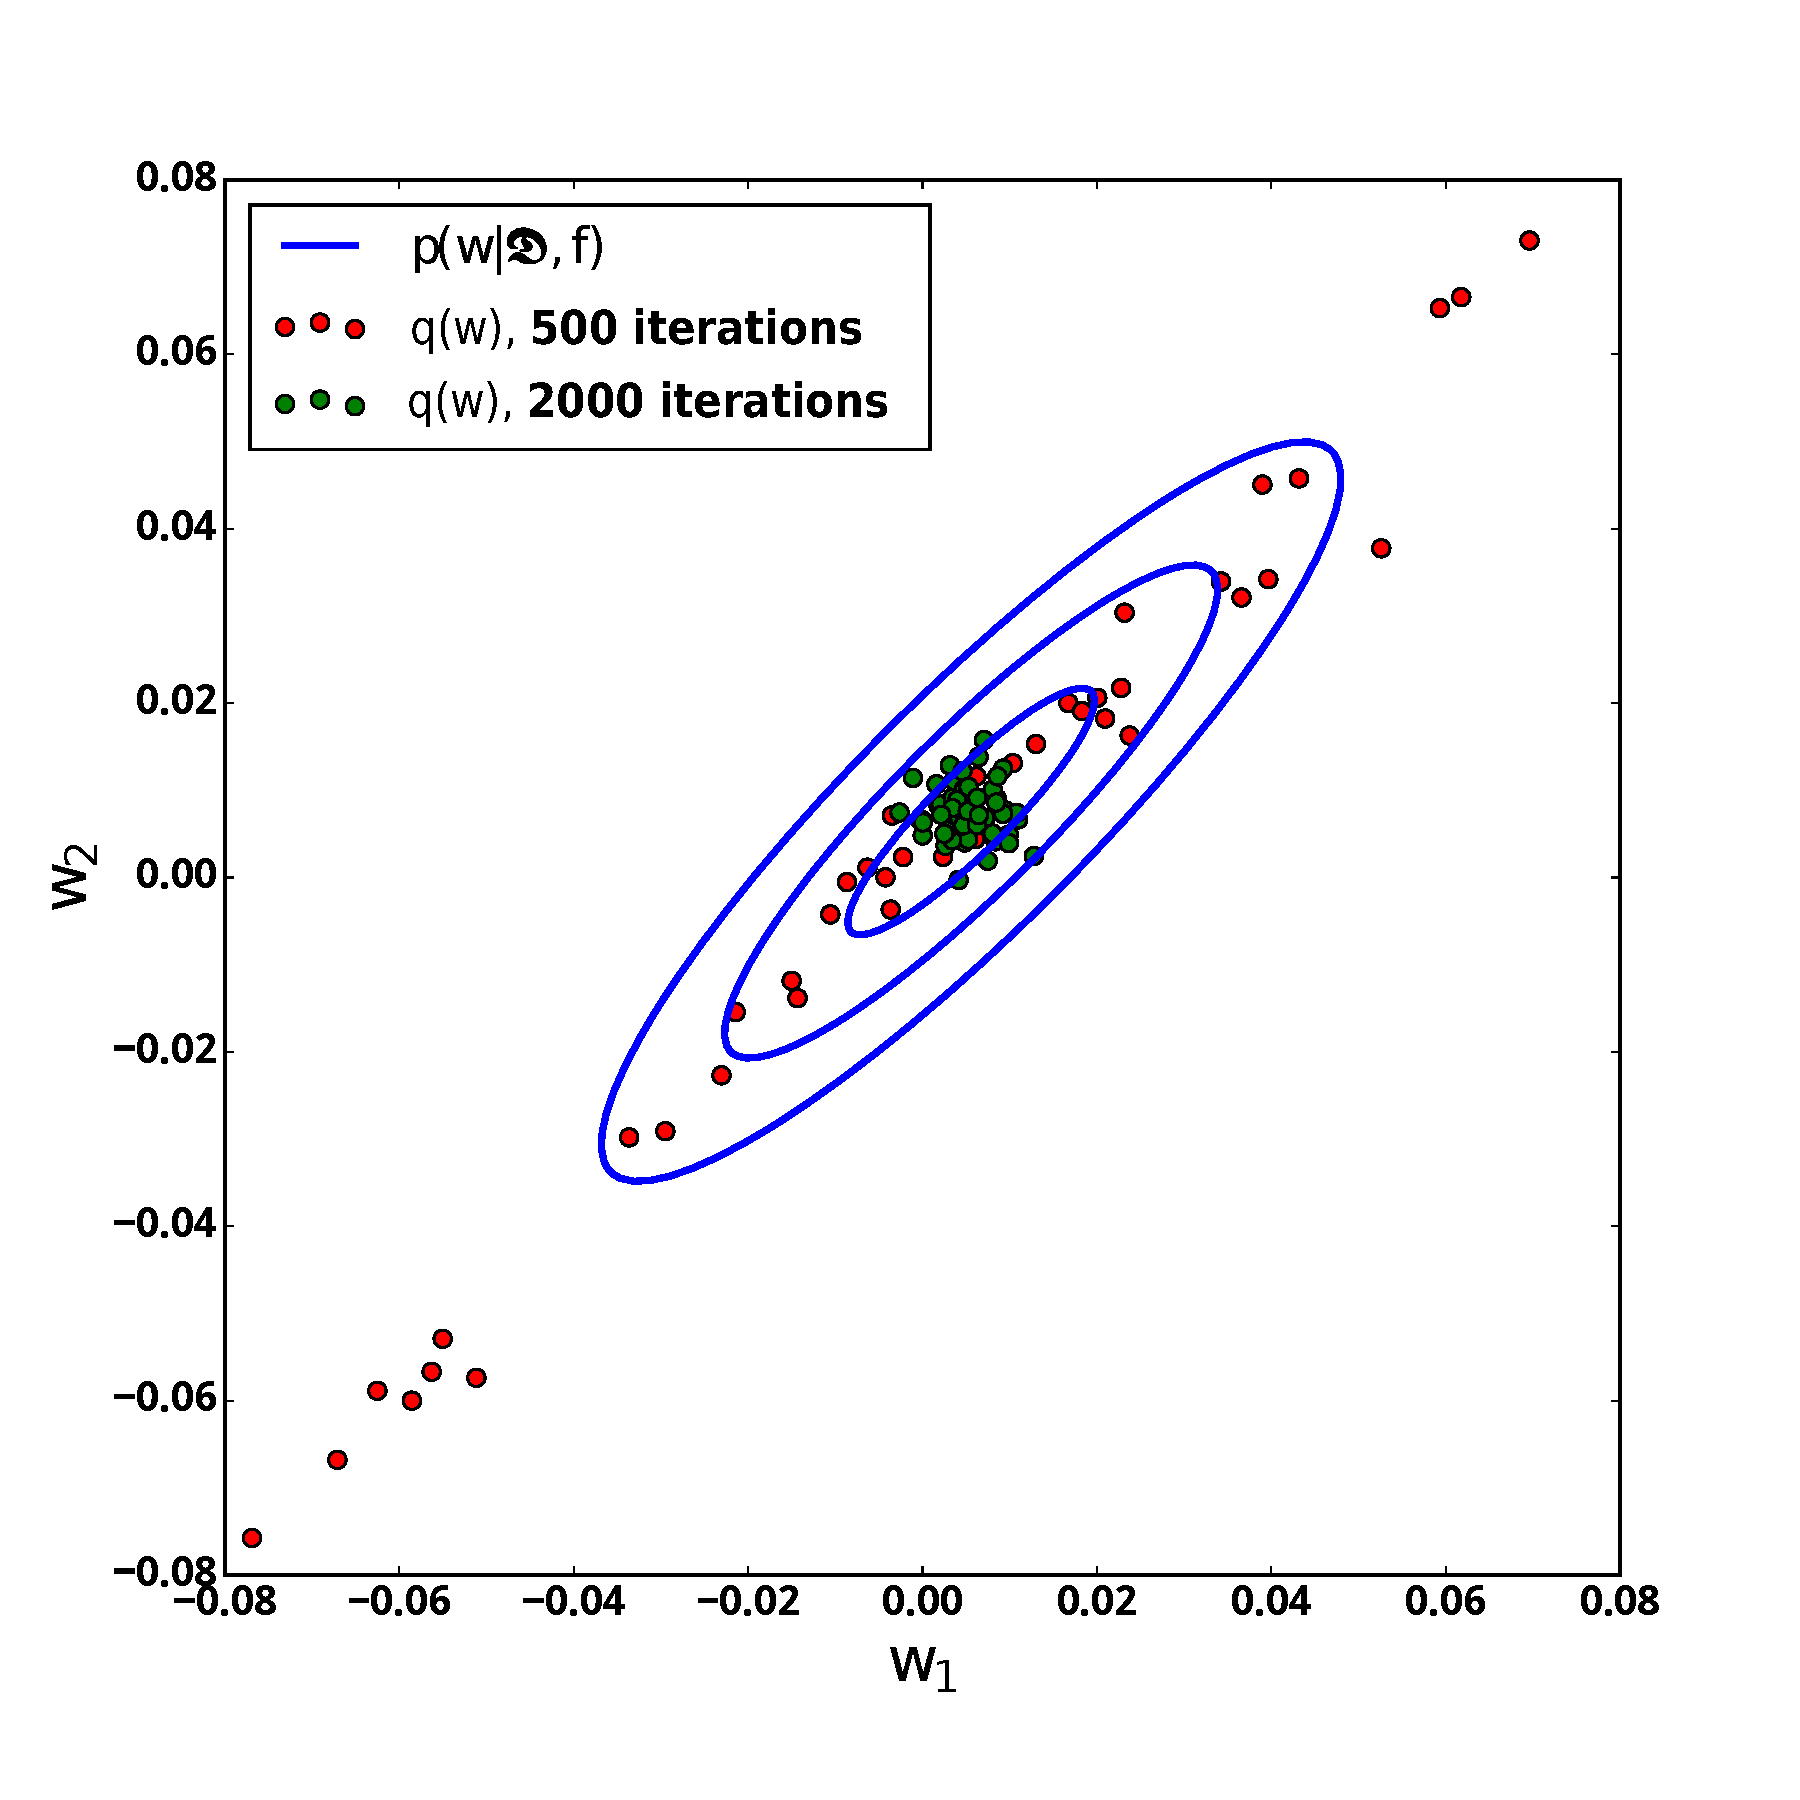
\includegraphics[width=0.52\textwidth]{./slide_plots/sgd_estimate_en.pdf}}
\end{figure}

\columnbreak

Evidence lower bound decrease is a signal of overfitting.
\vspace{-1.2cm}
\begin{figure}
{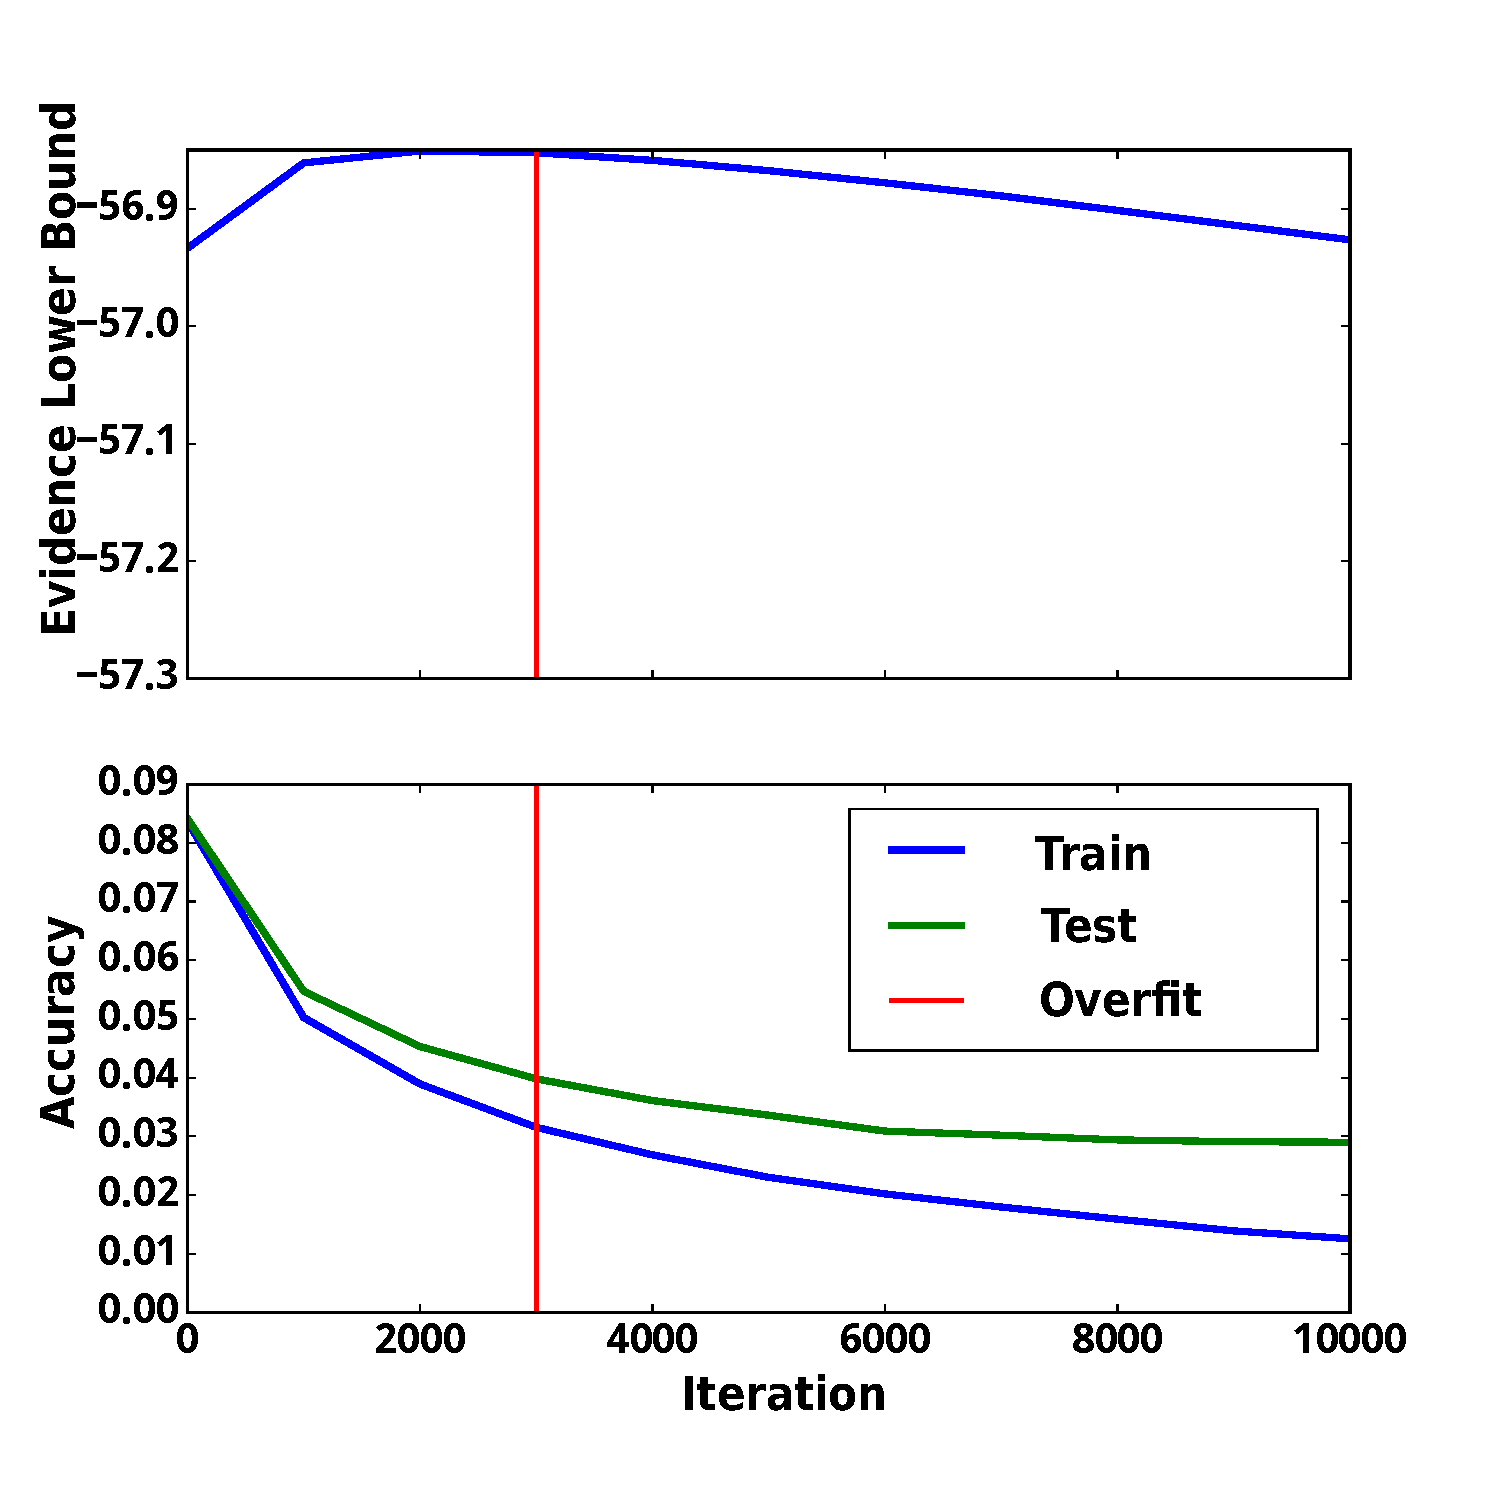
\includegraphics[width=0.52\textwidth]{./slide_plots/sgd_show_en.pdf}}
\end{figure}
\end{multicols}
\end{frame}










\begin{frame}{Proposed optimization analysis}
\footnotesize

\vspace{-0.1cm}
\begin{block}{Theorem, [Bakhteev, 2018]}
Let $\textcolor{red}{\lambda_\text{prior}^L} > 0, m \gg 0, \frac{m}{\lambda_\text{prior}^L} \in \mathbb{N}.$ Then optimization of \vspace{-0.3cm} \[L = 
\textcolor{blue}{\mathsf{E}_q \text{log}~{p(\mathbf{y} | \mathbf{X}, \mathbf{w}, \boldsymbol{\Gamma}, \mathbf{h}, \lambda_{\text{temp}},\mathbf{f})}} - \textcolor{red}{\lambda_\text{prior}^L\text{D}_{KL}(q||p(\mathbf{w}, \boldsymbol{\Gamma} |\mathbf{h}, \lambda_{\text{temp}, \mathbf{f}})))}\vspace{-0.2cm}\] is a minimization of  $\mathsf{E}_{\hat{\mathbf{X}}, \hat{\mathbf{y}}\sim p(\mathbf{X}, \mathbf{y})}\text{D}_{KL}(q||p(\mathbf{w}, \boldsymbol{\Gamma} | \hat{\mathbf{X}}, \hat{\mathbf{y}},\mathbf{h},\lambda_{\text{temp}},\mathbf{f})),$ where $\hat{\mathbf{X}}, \hat{\mathbf{y}}$ is a random sample of size  $\frac{m}{\textcolor{red}{\lambda_\text{prior}^L}}$.
\end{block}
\vspace{-0.2cm} 
\begin{block}{Definition}
Parametric complexity of the model is a minimal divergence:
\vspace{-0.2cm}
\[
    C_p = \min_{\mathbf{h}} \textcolor{red}{D_\text{KL}(q||p(\mathbf{w}, \boldsymbol{\Gamma}|\mathbf{h},\lambda_\text{temp}, \mathbf{f})).}
\]
\end{block}
\vspace{-0.2cm}
\begin{block}{Theorem, [Bakhteev, 2018]}
Let $\textcolor{OliveGreen}{\boldsymbol{\lambda}^Q_{\text{struct}}} = \bf 0$.
Let  $\teta_1, \teta_2, \h_1, \h_2$ are the optimization solutions for different metaparameter values $\textcolor{red}{{\lamCQ}_1,{\lamCQ}_2, {\lamCQ}_1>{\lamCQ}_2}$ on a compact $U$.
Let function $\Val$ be concave on  $U$ for $\textcolor{red}{{\lamCQ}_2}$.
Then:
\footnotesize
\vspace{-0.2cm}
\[
    C_p(\teta_1|\Uh, \lam_1) - C_p(\teta_2|\Uh, \lam_2)  < \frac{\lamCL }{{\lamCQ}_2} ({\lamCQ}_2- \lamCL) C,
\]
where $C$ is a constant.
\end{block}



\end{frame}



\begin{frame}{Proposed optimization analysis}
\vspace{-0.2cm} 
\begin{block}{Definition}
Relative variational density is a ratio:
\[
\rho(w|\boldsymbol{\Gamma},\boldsymbol{\theta}_\mathbf{w}, \mathbf{h},\boldsymbol{\lambda})=\frac{q_\mathbf{w}(\text{mode}~p(\mathbf{w}|\boldsymbol{\Gamma}, \mathbf{h}, \boldsymbol{\lambda}))}{q_\mathbf{w}(\text{mode}~{q_\mathbf{w}})}.
\]
\end{block}
\vspace{-0.2cm} 
\begin{block}{Theorem, [Bakhteev, 2018]}
Given $\Uh \subset \Hb, \Utetaw \subset \Tetawb, \UtetaG \subset \TetaGb$,
variational and prior distributions $\qw$, $\priorw$ are absolutely continuous and unimodal  $U_{\boldsymbol{\theta}}$  with equality of mode and mean.
Let mode and mean of prior distribution be independent on the hyperparameters $\h$ and the structure $\Gam$.\\
Given a infinite sequence $\teta[1],\teta[2],\dots,\teta[i],\dots \in \Uteta$ such that $\lim_{i \to \infty}C_p(\teta[i]|\Uh,\lam) = 0.$
Then
\footnotesize
$$
   \lim_{i \to \infty} \E_{\qG[][{\tetaG[i]}]} {\rho}(\w|\Gam, {\tetaw[i]}, {\h[i]}, \lam)^{-1} = 1, \h[i] = \argmin \KL{\q[\teta_i]}{\prior}.
$$
\end{block}


% 1. Заметим, что покомпонентная проекция выпулкых функций - выпукла (по определению вроде). поэтому L и Q можно рассматривать как большие мета-функции.
% 2. По условиям:  L_1(q1) - \lambda_1 DKL(q1) = max, L_2 - \lambda_2 DKL(q_2) = max.
% 3. L_1(q1) - \lambda_1 DKL(q1) - L_2(q2)  + \lambda_1 DKL(q2) >= 0
%    L_2(q2) - \lambda_2 DKL(q2) - L_1(q1) +  \lambda_2 DKL(q1) >= 0
% 4. Складываем
%    \lambda_1 DKL(q2) - \lambda_2DKL(q2) >= c1 DKL(q1) - c2 DKL(q1), DKL (q2) <= DKL(q1)
% 5. Заметим, что это DKL и есть параметрической сложностью.
% Пусть существует h': DKL(q|h')<DKL(q|h).
% Так как L не зависит от h, то получается что L-DKL|h' > L-DKL|h, противоречие.
\end{frame}


\begin{frame}{Main results}
\footnotesize
The following results were proposed:
\begin{enumerate}
\item method of Bayesian selection of suboptimal structure;
\item optimal and suboptimal complexity criteria;
\item deep learning model graph description;
\item generalizing function that includes other methods of model selection:
\begin{itemize}
\footnotesize
\item evidence lower bound;
\item sequential complexity increase;
\item sequential complexity decrease;
\item structure exhaustive search;
\end{itemize}


\item method of evidence lower bound optimization based on mutlistart model optimization;
\item algorithm of optimization hyperparameters, structure and parameters for deep learning model.
\item The properties of the proposed optimization were investigated and comprehensively analyzed.

\end{enumerate}
\end{frame}



\begin{frame}{Publications}
\tiny
\textbf{Main publications}
\begin{enumerate}
\item Bakhteev, O., Kuznetsova, R., Romanov, A. and Khritankov, A. A monolingual approach to detection of text reuse in Russian-English collection // In 2015 Artificial Intelligence and Natural Language and Information Extraction, Social Media and Web Search FRUCT Conference (AINL-ISMW FRUCT) (pp. 3-10). IEEE.

\item Бахтеев О.Ю., Попова М.С., Стрижов В.В. Системы и средства глубокого обучения в задачах классификации. // Системы и средства информатики. 2016. № 26.2. С. 4-22.
\item Romanov, A., Kuznetsova, R., Bakhteev, O. and Khritankov, A. Machine-Translated Text Detection in a Collection of Russian Scientific Papers. // Computational Linguistics and Intellectual Technologies. 2016. 
\item Bakhteev, O. and Khazov, A., 2017. Author Masking using Sequence-to-Sequence Models // In CLEF (Working Notes). 2017.
\item Бахтеев О.Ю., Стрижов В.В. Выбор моделей глубокого обучения субоптимальной сложности. // Автоматика и телемеханика. 2018. №8. С. 129-147.
\item Огальцов А.В., Бахтеев О.Ю. Автоматическое извлечение метаданных из научных PDF-документов. // Информатика и её применения. 2018.
\item Смердов А.Н., Бахтеев О.Ю., Стрижов В.В. Выбор оптимальной модели рекуррентной сети в задачах поиска парафраза. // Информатика и ее применения. 2019.
\item Грабовой А.В., Бахтеев О.Ю., Стрижов В.В. Определение релевантности параметров нейросети. // Информатика и её применения. 2019.
\item Bakhteev O., Strijov V. Comprehensive analysis of gradient-based hyperparameter optimization algorithms // Annals of Operations Research. 2019.
\end{enumerate}
\textbf{Conference talks}
\begin{enumerate}
\item ``Восстановление панельной матрицы и ранжирующей модели в разнородных шкалах'', Всероссийская конеренция <<57-я научная конеренция МФТИ>>, 2014.
\item ``Выбор модели глубокого обучения субоптимальной сложности с использованием вариационной оценки правдоподобия'', Международная конференция <<Интеллектуализация обработки информации>>, 2016.
\item ``Градиентные методы оптимизации гиперпараметров моделей глубокого обучения'', Всероссийская конференция <<Математические методы распознавания образов ММРО>>, 2017.
\item ``Детектирование переводных заимствований в текстах научных статей из журналов, входящих в РИНЦ'', Всероссийская конференция <<Математические методы распознавания образов ММРО>>, 2017.
\item ``Байесовский выбор наиболее правдоподобной структуры модели глубокого обучения'', Международная конференция <<Интеллектуализация обработки информации>>, 2018.
\end{enumerate}
\end{frame}





\end{document}
